% =============================================================================
% Chuong 5: Thuc nghiem va danh gia (chuan lop article cho Internship2_HK262)
% =============================================================================

\chapter{Thực nghiệm và đánh giá}
\label{ch:thuc-nghiem}

Chương này kiểm chứng toàn diện đề xuất \CTAV{} và tác tử RCA theo trình tự thực nghiệm ba lớp: kiểm tra tính đúng của pipeline cơ sở và khả năng tái lập hồi quy (Mục~\ref{sec:ch5-gates}), tinh chỉnh và chọn cấu hình trên tập \splitname{val} (Mục~\ref{sec:ch5-val}), cuối cùng kiểm định một lần duy nhất trên tập \splitname{test} đã niêm phong cho cả nhánh thẩm định cảnh báo lẫn nhánh phân tích nguyên nhân gốc (Mục~\ref{sec:ch5-test}--\ref{sec:ch5-rca}). Mở đầu chương, các mục từ~\ref{sec:ch5-hypotheses} đến~\ref{sec:ch5-metrics} trình bày sáu giả thuyết đăng ký trước H0--H5, giao thức chia dữ liệu chống rò rỉ, thiết lập thực nghiệm và hệ thống thước đo. Mục~\ref{sec:ch5-synthesis} tổng hợp mười hai phát hiện thực nghiệm định hình các quyết định thiết kế, và Mục~\ref{sec:ch5-ket-chuong} tóm tắt kết luận kiểm định trước khi chuyển sang phần trình diễn nền tảng ở Chương~\ref{ch:platform}.

% -----------------------------------------------------------------------------
\section{Mục tiêu thực nghiệm và các giả thuyết H0--H5}
\label{sec:ch5-hypotheses}

Thực nghiệm của đề tài hướng tới hai mục tiêu định lượng đã xác lập ở Chương~\ref{ch:mo-dau}: (A) kiểm chứng liệu \CTAV{} có duy trì mức tăng thu hồi (recall) của truy xuất nhận biết topology mà không làm tăng tỷ lệ báo động giả (FPR) so với truy xuất từ khóa cục bộ BM25 trong cùng ngân sách gọi LLM hay không; và (B) kiểm chứng liệu tác tử RCA đứng sau \CTAV{} có định vị được service gốc, giảm số cảnh báo qua gom sự cố và sinh báo cáo chẩn đoán hợp lệ hay không.

Để ngăn ngừa tinh chỉnh hậu nghiệm, toàn bộ sáu giả thuyết H0--H5 cùng tiêu chí chấp nhận và cấu hình đóng băng đã được đăng ký công khai trong kho mã nguồn tại một commit riêng (\code{be2b985}) trước bất kỳ lượt chạy nào trên tập \splitname{test}. Quy ước thống kê áp dụng đồng nhất gồm: khoảng tin cậy 95\% (CI95) ước lượng bằng bootstrap phân vị 1.000 mẫu (\code{seed = 42}) và kiểm định McNemar chính xác hai phía ở mức ý nghĩa $\alpha = 0{,}05$. Trong đó, \textbf{H2} là giả thuyết chính; các giả thuyết H0, H3, H4 là giả thuyết phụ, báo giá trị $p$ thô không hiệu chỉnh đa so sánh. Chỉ số chính của nhánh thẩm định tính trên tập con \emph{cửa sổ có telemetry}; kết quả trên toàn bộ split được báo làm chỉ số phụ. Bảng~\ref{tab:h0-h5} liệt kê nguyên văn tiêu chí chấp nhận đã đăng ký cho H0--H5.

\begin{table}[htbp]
  \centering
  \caption[Giả thuyết H0--H5 và tiêu chí chấp nhận đã đăng ký]{Hệ thống giả thuyết H0--H5 và tiêu chí chấp nhận đã đăng ký trước khi chạm tập \splitname{test}.}
  \label{tab:h0-h5}
  \scriptsize
  \renewcommand{\arraystretch}{1.15}
  \setlength{\tabcolsep}{3.5pt}
  \begin{tabularx}{\linewidth}{@{}l >{\raggedright\arraybackslash}p{3.6cm} Y >{\raggedright\arraybackslash}p{2.3cm}@{}}
    \toprule
    \textbf{Mã} & \textbf{Nội dung giả thuyết} & \textbf{Tiêu chí chấp nhận đã đăng ký (\code{be2b985})} & \textbf{Phạm vi kiểm} \\
    \midrule
    \textbf{H0} & Topology chưa hiệu chỉnh (C1) tăng recall và tăng FPR so với BM25 & CI95 của $\Delta\text{Recall}$ và $\Delta\text{FPR}$ có cận dưới $> 0$; McNemar trên cửa sổ lỗi và bình thường đều $p < 0{,}05$ & \splitname{val} \& \splitname{test} \\
    \textbf{H1} & Cơ chế: \code{TRUE\_ALERT} trên cửa sổ bình thường tăng theo độ gần thời gian và loại bằng chứng (trace) & Xu hướng đơn điệu dương kèm CI95 trên mẫu can thiệp cố định; không chạy lại trên \splitname{test} & Chỉ \splitname{val} \\
    \textbf{H2} (chính) & \CTAV{} tốt hơn BM25 và giữ phần lớn recall của C1 & (i)~CI95 $\Delta\text{F1}(\text{\CTAV}-\text{BM25})$ cận dưới $> 0$ và McNemar $p < 0{,}05$; (ii)~CI95 $\Delta\text{FPR}(\text{\CTAV}-\text{BM25})$ không có cận dưới $> 0$; (iii)~ước lượng điểm $\Delta\text{Recall}(\text{\CTAV}-\text{C1}) \ge -0{,}05$. Đạt (i)--(ii) nhưng trượt (iii) $\Rightarrow$ ``đạt một phần'' & \splitname{val} (sơ bộ) \& \splitname{test} \\
    \textbf{H3} & Đóng góp từng thành phần quanh \CTAV{} (một-thay-đổi-một-lần) & Bỏ C3 $\Rightarrow$ CI95 $\Delta\text{Precision}$ cận trên $< 0$; thêm C2 xác nhận loại nếu CI95 $\Delta\text{FPR}$ chứa $0$ hoặc $> 0$; thêm C4 xác nhận loại nếu chi phí tăng và CI95 $\Delta\text{F1}$ không có cận dưới $> 0$; báo mô tả C3-trượt và C5 một điểm & \splitname{val} \& \splitname{test} \\
    \textbf{H4} & Ở ngân sách 120 lần gọi, \CTAV{} không kém LLM-không-RAG & Ước lượng điểm $\text{F1}(\text{\CTAV}) \ge \text{F1}(\text{không-RAG})$ ở mốc 120 lần gọi; báo kèm toàn bộ đường ngân sách & \splitname{val} \& \splitname{test} \\
    \textbf{H5} & Tác tử RCA định vị service gốc và giảm cảnh báo & $\text{Hit@1} \ge 0{,}60$, $\text{Hit@3} \ge 0{,}80$, cận dưới CI95 của $\Delta\text{Hit@1}(\text{RCA}-\text{baseline}) > 0$, và Alert Reduction $\ge 30\%$ trên sự cố cascade & \splitname{val} \& \splitname{test} \\
    \bottomrule
  \end{tabularx}
\end{table}

% -----------------------------------------------------------------------------
\section{Dữ liệu và giao thức chia split chống rò rỉ}
\label{sec:ch5-data}

Toàn bộ thí nghiệm sử dụng bộ dữ liệu microservice đa phương thức công khai Nezha~\cite{yu2023nezha} (gồm hai hệ thống OnlineBoutique và TrainTicket với năm loại lỗi tiêm có chủ đích: \code{network\_delay}, \code{cpu\_contention}, \code{cpu\_consumed}, \code{exception}, \code{return}). Đồ thị phụ thuộc service dựng từ cặp \code{SpanID}--\code{ParentID} của trace gồm $56$ service và $68$ cạnh có hướng. Dữ liệu được cắt thành các cửa sổ không chồng lấn độ dài $60\,\text{s}$ và gán nhãn theo thời gian thực (\emph{wall-clock}) như trình bày ở Mục~\ref{sec:ch2-du-lieu}.

Để loại bỏ rò rỉ dữ liệu theo thời gian và theo cùng một sự cố, đề tài áp dụng giao thức chia ba tập \splitname{dev}, \splitname{val}, \splitname{test} cố định bằng \code{seed = 42}, minh họa ở Hình~\ref{fig:ch5-split}. Toàn bộ $7$ cửa sổ của mỗi lần tiêm lỗi (\code{injection\_id}) luôn nằm trọn trong cùng một split; $597$ cửa sổ bình thường của cùng pod nằm trong vùng đệm $600\,\text{s}$ quanh thời điểm tiêm lỗi bị loại bỏ để tránh dính dư chấn lỗi; các cửa sổ bình thường còn lại được phân bổ nguyên khối theo cặp \code{ngày|pod} và \emph{không lấy mẫu giảm bớt} (giữ nguyên tỷ lệ mất cân bằng tự nhiên xấp xỉ $1:135$). Trong đó, \splitname{dev} chỉ dùng để huấn luyện bộ phát hiện, dựng ngưỡng nền C3 và gỡ lỗi; \splitname{val} dùng để chạy H1 và chọn cấu hình; \splitname{test} bị niêm phong và chỉ chạy một lần sau khi đăng ký giả thuyết.

\begin{figure}[htbp]
  \centering
  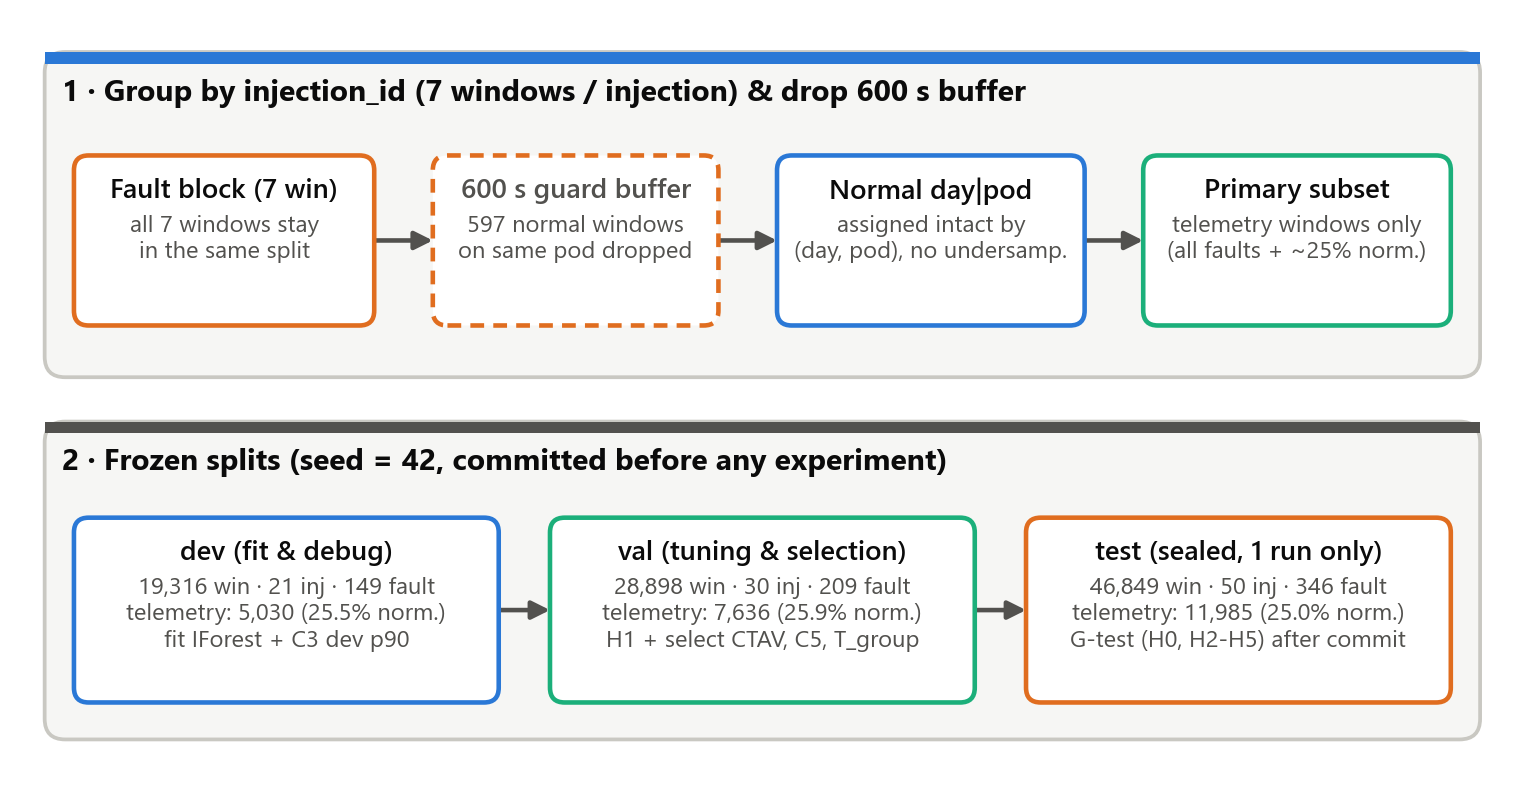
\includegraphics[width=\linewidth]{figures/ch5/h5.1-split-protocol.png}
  \caption[Giao thức chia dữ liệu chống rò rỉ theo lần tiêm lỗi]{Giao thức chia split chống rò rỉ trên Nezha: giữ nguyên khối 7 cửa sổ mỗi lần tiêm lỗi, loại vùng đệm 600~s và khóa cứng ba tập \splitname{dev}, \splitname{val}, \splitname{test}. \emph{(Nguồn: tác giả vẽ, có hỗ trợ AI.)}}
  \label{fig:ch5-split}
\end{figure}

Bảng~\ref{tab:ch5-splits} thống kê kích thước ba split, đồng thời chỉ ra một đặc điểm cấu trúc quan trọng của Nezha (\textbf{Phát hiện 1}): bộ dữ liệu chỉ lưu tệp log và trace xung quanh các khoảng thời gian tiêm lỗi. Mọi cửa sổ lỗi ($100\%$) đều có dữ liệu log hoặc trace, trong khi chỉ khoảng $25\%$ cửa sổ bình thường có telemetry kèm theo. Trên tập đối chiếu mẫu nhỏ của nghiên cứu tiền đề~\cite{author2026icaetm}, khảo sát độ phủ ở Bảng~\ref{tab:ch5-coverage} cho thấy chỉ $5{,}4\%$ cửa sổ bình thường truy xuất được bằng chứng khác rỗng trong kho đã lọc theo nhãn ($19{,}4\%$ trong kho đầy đủ), đồng nghĩa sự hiện diện của bằng chứng gần như trùng khớp với dấu hiệu gần sự cố. Để tránh việc bộ thẩm định thắng giả nhờ từ chối các cửa sổ thiếu dữ liệu, tập chấm chính của đề tài được giới hạn trên các \emph{cửa sổ có telemetry} ($5.030$ cửa sổ trên \splitname{dev}, $7.636$ trên \splitname{val} và $11.985$ trên \splitname{test}).

\begin{table}[htbp]
  \centering
  \caption[Kích thước các split và tỷ lệ cửa sổ có telemetry trên Nezha]{Kích thước ba split \splitname{dev}, \splitname{val}, \splitname{test} và tỷ lệ cửa sổ có dữ liệu telemetry đi kèm.}
  \label{tab:ch5-splits}
  \scriptsize
  \renewcommand{\arraystretch}{1.15}
  \begin{tabularx}{\linewidth}{@{}l r r r r Y@{}}
    \toprule
    \textbf{Split} & \textbf{Tổng cửa sổ} & \textbf{Cửa sổ lỗi} & \textbf{Lần tiêm lỗi} & \textbf{Lỗi có telemetry} & \textbf{Bình thường có telemetry} \\
    \midrule
    \splitname{dev} & 19.316 & 149 & 21 & 149 / 149 (100\%) & 4.881 / 19.167 (25,5\%) \\
    \splitname{val} & 28.898 & 209 & 30 & 209 / 209 (100\%) & 7.427 / 28.689 (25,9\%) \\
    \splitname{test} & 46.849 & 346 & 50 & 346 / 346 (100\%) & 11.639 / 46.503 (25,0\%) \\
    \bottomrule
  \end{tabularx}
\end{table}

\begin{table}[htbp]
  \centering
  \caption[Độ phủ bằng chứng giữa cửa sổ lỗi và cửa sổ bình thường]{Độ phủ bằng chứng trên tập mẫu đối chiếu ($98$ cửa sổ lỗi, $391$ cửa sổ bình thường), làm rõ động lực chọn tập chấm chính trên cửa sổ có telemetry.}
  \label{tab:ch5-coverage}
  \scriptsize
  \renewcommand{\arraystretch}{1.15}
  \begin{tabularx}{\linewidth}{@{}Y r r@{}}
    \toprule
    \textbf{Điều kiện tồn tại bằng chứng} & \textbf{Cửa sổ lỗi (98)} & \textbf{Cửa sổ bình thường (391)} \\
    \midrule
    Kho đối chiếu lọc theo nhãn: top-6 khác rỗng & 89 (90,8\%) & 21 (5,4\%) \\
    Kho Nezha đầy đủ: top-6 khác rỗng & 98 (100,0\%) & 76 (19,4\%) \\
    Có tệp log hoặc trace trong biên $\pm 8$ phút & 98 (100,0\%) & 106 (27,1\%) \\
    \bottomrule
  \end{tabularx}
\end{table}

% -----------------------------------------------------------------------------
\section{Thiết lập thực nghiệm và chi phí}
\label{sec:ch5-setup}

Mọi thí nghiệm thẩm định chính thức sử dụng một mô hình API duy nhất là \code{gemini-2.5-flash} ở nhiệt độ $0$, tắt vùng suy luận ẩn (\code{thinkingBudget = 0}), bỏ cột metric hằng lỗi \code{PodSuccessRate(\%)} khỏi prompt (\textbf{Phát hiện 5}), và đi qua lớp cache JSONL khóa \code{sha256} (Mục~\ref{sec:ch4-judge}). Riêng cổng kiểm chứng hồi quy G-paper đọc lại trực tiếp tệp cache của mô hình \code{gemini-2.5-flash-lite} với tỷ lệ trúng cache $100\%$. Bộ phát hiện Isolation Forest (ngưỡng $0{,}85$, \code{buffer\_size = 2}) được huấn luyện duy nhất trên \splitname{dev}. Truy xuất C1 sử dụng cấu hình $\alpha = 0{,}35$, $\beta = 0{,}25$, $\gamma = 0{,}40$, $\tau_F = 300\,\text{s}$, mở rộng $2$ hop, top-$6$ trong $4.000$ token với engine vector hóa (trung bình $\approx 0{,}45\,\text{s}$ mỗi truy vấn).

Các lượt gọi API chạy song song 8 luồng với bộ giới hạn tốc độ 200 lượt gọi/phút; toàn bộ đánh giá \CTAV{} và các nhánh loại trừ H3 được thực hiện bằng chế độ phát lại trên phán quyết đã lưu cache (\code{py -m eval ctav}, chi phí $0$ USD). Bảng~\ref{tab:ch5-costs} tổng hợp chi phí ước tính theo đơn giá token của toàn bộ chiến dịch thực nghiệm; lưu ý đây là chi phí quy đổi từ số lượng token ghi trong sổ cái cache, chưa đối chiếu trực tiếp với hóa đơn thanh toán cuối cùng của nhà cung cấp.

\begin{table}[htbp]
  \centering
  \caption[Tổng hợp chi phí gọi API LLM theo các hạng mục thực nghiệm]{Chi phí gọi API LLM ước tính theo sổ cái token cho từng hạng mục thực nghiệm chính.}
  \label{tab:ch5-costs}
  \scriptsize
  \renewcommand{\arraystretch}{1.15}
  \begin{tabularx}{\linewidth}{@{}l Y r Y@{}}
    \toprule
    \textbf{Hạng mục} & \textbf{Nội dung chạy chính} & \textbf{USD theo token} & \textbf{Ghi chú} \\
    \midrule
    Kiểm chứng G-port / G-paper & Khớp pipeline mock + tái lập 489 ca từ cache + smoke test & 0,29 & G-paper đạt 100\% cache hit (0 USD) \\
    Thực nghiệm H0 trên \splitname{val} & BM25, C1 ($k_{\text{graph}} \in \{0, 1\}$), LLM-không-RAG & $\approx 8{,}60$ & Có phần tái sử dụng cache giữa các nhánh \\
    Thí nghiệm cơ chế H1 trên \splitname{val} & 9 điều kiện can thiệp (6.988 lượt gọi thành công) & 9,48 & Dùng mẫu cố định 1.749 candidate \\
    Chọn cấu hình \CTAV{} & Replay toàn bộ chính sách và ablation H3 trên \splitname{val} & 0,00 & Mô phỏng C1 mọi candidate $\approx 3{,}28$ USD/run \\
    Khảo sát C5 trên \splitname{val} & Chấm một lần 1.459 cửa sổ được cứu & 1,03 & Quét 147 điểm lưới ngoại tuyến \\
    Kiểm định G-test trên \splitname{test} & BM25, C1, không-RAG, C5 một điểm, 4 run \code{repeat} & 15,85 & 21.094 lượt gọi API mới, 0 lỗi judge \\
    Tác tử RCA (\splitname{val} \& \splitname{test}) & Tóm tắt 26 (\splitname{val}) + 38 (\splitname{test}) + 114 (độ nhạy) sự cố & 0,28 & Tổng 178 lượt gọi, 0 báo cáo bị loại \\
    \bottomrule
  \end{tabularx}
\end{table}

% -----------------------------------------------------------------------------
\section{Thước đo đánh giá}
\label{sec:ch5-metrics}

Các công thức định nghĩa thước đo đã được trình bày ở Mục~\ref{sec:ch2-danh-gia}; mục này chốt quy ước áp dụng thống nhất cho toàn chương:
\begin{itemize}
  \item \emph{Nhánh thẩm định cảnh báo:} Báo cáo \code{TP}, \code{FP}, Precision, Recall, F1 (lấy 3 chữ số thập phân) và FPR (lấy 4 chữ số thập phân do FPR của \CTAV{} ở hàng phần nghìn). Recall luôn tính trên \emph{tổng số cửa sổ lỗi của split} (kể cả cửa sổ bị bộ phát hiện bỏ sót); trạng thái \code{UNCERTAIN} và \code{manual\_review} không tính là cảnh báo phát ra.
  \item \emph{Kiểm định thống kê và độ ổn định:} Mọi hiệu ghép cặp $\Delta = \text{phương pháp} - \text{đối chứng}$ kèm CI95 bootstrap 1.000 mẫu (\code{seed = 42}) và giá trị $p$ của kiểm định McNemar chính xác tách riêng trên cửa sổ lỗi và cửa sổ bình thường. Độ ổn định của judge được đo bằng tỷ lệ lật phán quyết qua ba lần gọi độc lập \code{repeat} $\in \{0, 1, 2\}$ trên tập con 200 candidate.
  \item \emph{Nhánh phân tích nguyên nhân gốc:} Đánh giá $\text{Hit@1}$, $\text{Hit@3}$ trên các sự cố có nhãn đơn lỗi (loại sự cố đa lỗi nhập nhằng \code{ambiguous} và báo rõ số lượng), đối chiếu với baseline xếp hạng theo điểm bất thường cao nhất; đo \emph{Alert Reduction Ratio} ($\text{ARR} = 1 - \text{\#sự cố}/\text{\#cảnh báo}$), tỷ lệ JSON hợp lệ (\emph{JSON valid rate}) và độ trễ hồi phát.
\end{itemize}

% -----------------------------------------------------------------------------
\section{Kiểm chứng tính đúng của pipeline và tái lập hồi quy}
\label{sec:ch5-gates}

Trước khi chạy các thí nghiệm khoa học trên giao thức chống rò rỉ mới, hệ thống phải vượt qua hai cổng kiểm chứng kỹ thuật là G-port và G-paper (đặt trên cùng trục ba cổng kiểm chứng với G-test ở Hình~\ref{fig:ch5-gates}).

\begin{figure}[htbp]
  \centering
  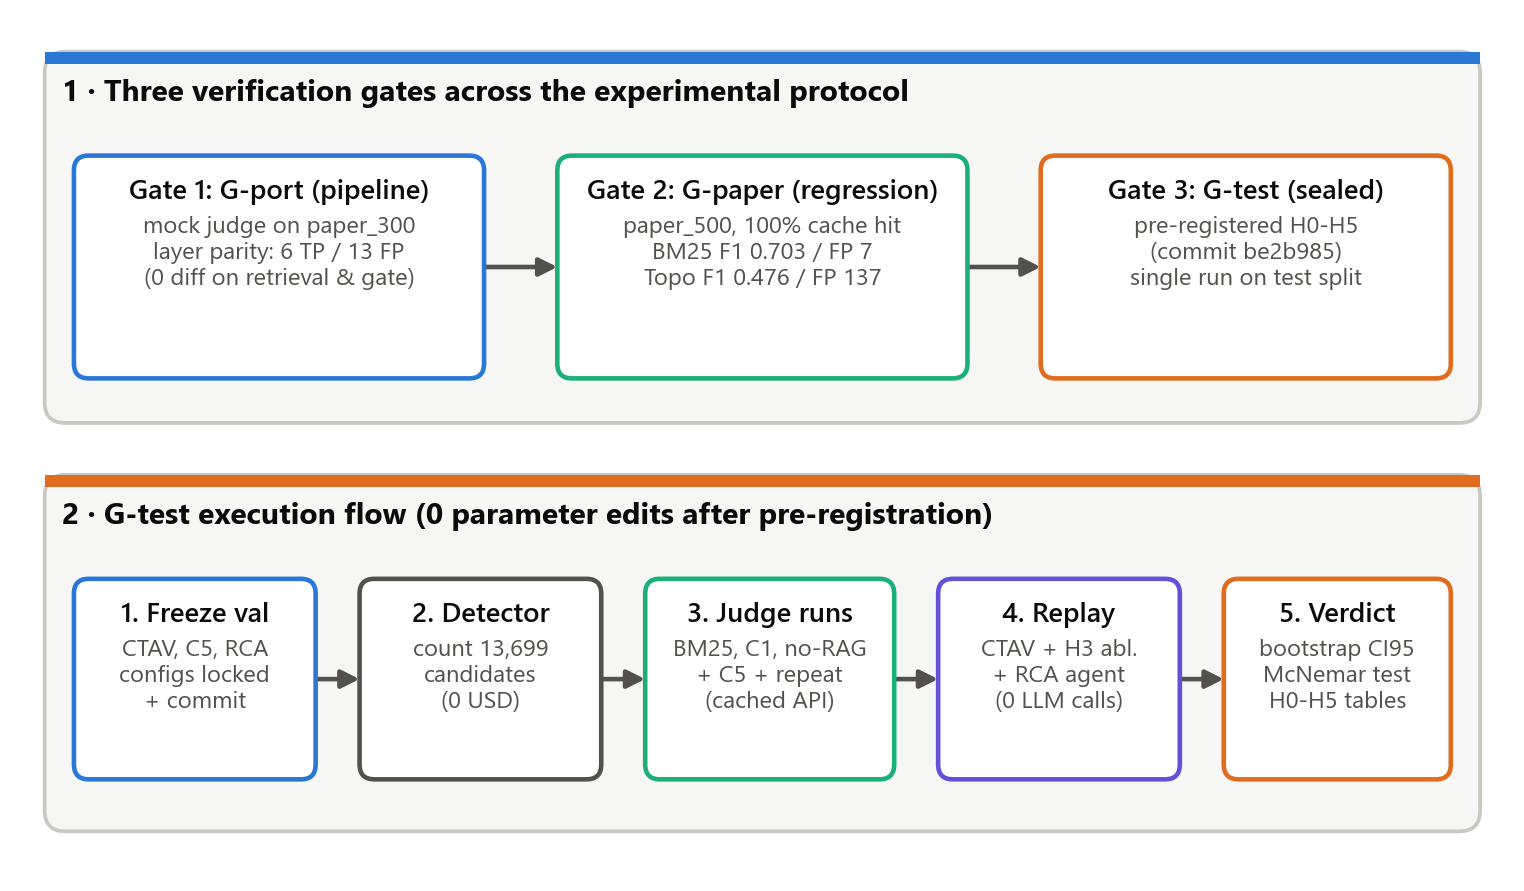
\includegraphics[width=\linewidth]{figures/ch5/h5.3-three-gates.png}
  \caption[Ba cổng kiểm chứng kỹ thuật và luồng thực thi G-test]{Ba cổng kiểm chứng thực nghiệm (G-port, G-paper, G-test) và quy trình năm bước khép kín của G-test sau khi đăng ký trước giả thuyết tại commit \code{be2b985}. \emph{(Nguồn: tác giả vẽ, có hỗ trợ AI.)}}
  \label{fig:ch5-gates}
\end{figure}

\subsection{Kiểm chứng pipeline cơ sở (G-port)}
\label{sec:ch5-gport}

Cổng G-port đối chiếu hành vi từng tầng của pipeline hiện thực với bản tham chiếu đã chốt bằng bộ thẩm định giả lập (\emph{mock judge}) trên tập \code{paper\_300} (ngưỡng $0{,}95$, cổng tin cậy $0{,}80 / 0{,}98$, ngân sách $30$ lượt gọi; kết quả tham chiếu: Precision $0{,}3158$ với $6$ TP / $13$ FP, Recall $0{,}375$, FPR $0{,}0458$). Kết quả kiểm chứng phân rã theo từng tầng ở Bảng~\ref{tab:ch5-gport} cho thấy ba tầng lõi — truy xuất BM25 ($40/40$ top-6 trùng), bộ thẩm định giả lập ($30/30$) và tầng cổng ngân sách khi nhận cùng đầu vào ứng viên ($6$ TP / $13$ FP / $10$ FN / $271$ TN) — khớp tuyệt đối $100\%$. Khi chạy toàn pipeline với bộ phát hiện Isolation Forest mới trên cửa sổ $60\,\text{s}$, số FP lệch $+6$ ($6/19/10/265$, tương quan thứ hạng Spearman $0{,}79$) do sự khác biệt tự nhiên của đặc trưng bộ đệm cuộn; kiểm chứng cho thấy $10/13$ FP ở bản tham chiếu phát sinh từ luật ``hết ngân sách tự động đẩy cảnh báo'', không phải từ bộ thẩm định. Cổng G-port được xác nhận đạt theo tầng; các con số với bộ thẩm định giả lập chỉ phục vụ kiểm chứng phần mềm và không dùng để rút kết luận khoa học.

\begin{table}[htbp]
  \centering
  \caption[Kết quả kiểm chứng pipeline cơ sở G-port theo từng tầng]{Kiểm chứng từng tầng của cổng G-port trên tập \code{paper\_300} (dùng bộ thẩm định giả lập, chỉ kiểm chứng tính đúng kỹ thuật).}
  \label{tab:ch5-gport}
  \scriptsize
  \renewcommand{\arraystretch}{1.15}
  \begin{tabularx}{\linewidth}{@{}l Y l@{}}
    \toprule
    \textbf{Tầng kiểm chứng} & \textbf{Kết quả đo được} & \textbf{Đánh giá} \\
    \midrule
    1. Truy xuất BM25 & Top-6 trùng khớp tuyệt đối $40/40$ truy vấn & Đạt \\
    2. Bộ thẩm định giả lập (mock) & Phán quyết trùng khớp tuyệt đối $30/30$ ca & Đạt \\
    3a. Cổng ngưỡng \& ngân sách (cùng đầu vào ứng viên) & Ma trận nhầm lẫn $6/13/10/271$ trùng tuyệt đối bản tham chiếu & Đạt \\
    3b. Toàn pipeline với bộ phát hiện cửa sổ 60~s & $6/19/10/265$ (lệch $+6$ FP; Spearman điểm detector $0{,}79$) & Chấp nhận theo tầng \\
    \bottomrule
  \end{tabularx}
\end{table}

\subsection{Kiểm chứng hồi quy trên tập đối chiếu (G-paper)}
\label{sec:ch5-gpaper}

Cổng G-paper kiểm tra khả năng tái lập chính xác hai mốc baseline đã công bố trong khảo sát bước đầu~\cite{author2026icaetm} trên tập \code{paper\_500} ($100$ cửa sổ lỗi, $400$ cửa sổ bình thường, mô hình \code{gemini-2.5-flash-lite}, ngân sách đầy đủ) hoàn toàn từ lớp cache mà không phát sinh bất kỳ lượt gọi API mới nào. Như trình bày trong Bảng~\ref{tab:ch5-gpaper}, cả hai chiến lược BM25 và Topology đều khớp $489/489$ truy vấn về top-6 bằng chứng, chuỗi prompt và khóa cache ($100\%$ cache hit), tái lập chính xác từng con số đã công bố (BM25 đạt F1 $0{,}7030$ với $7$ FP; Topology đạt F1 $0{,}4759$ với $137$ FP).

\begin{table}[htbp]
  \centering
  \caption[Kết quả kiểm chứng hồi quy G-paper trên tập đối chiếu]{Kiểm chứng hồi quy G-paper trên \code{paper\_500} (\code{gemini-2.5-flash-lite}, tỷ lệ trúng cache $100\%$, $0$ lượt gọi API mới).}
  \label{tab:ch5-gpaper}
  \scriptsize
  \renewcommand{\arraystretch}{1.15}
  \begin{tabularx}{\linewidth}{@{}l Y r r r r r@{}}
    \toprule
    \textbf{Biến thể} & \textbf{Khớp top-6 / prompt / cache} & \textbf{TP} & \textbf{FP} & \textbf{Precision} & \textbf{Recall} & \textbf{F1 (công bố)} \\
    \midrule
    BM25 & $489/489/489$ & 58 & 7 & 0,8923 & 0,580 & 0,7030 (0,7030) \\
    Topology & $489/489/489$ & 74 & 137 & 0,3507 & 0,740 & 0,4759 (0,4759) \\
    \bottomrule
  \end{tabularx}
\end{table}

Quá trình giải phẫu cổng G-paper đồng thời bộc lộ ba phát hiện nền tảng về giao thức cũ: độ tin cậy mô hình trả ra phần lớn sao chép trực tiếp từ \code{anomaly\_score} khi thiếu ngữ cảnh (\textbf{Phát hiện 2}); biến thể ``topology'' trên tập mẫu cũ thực chất hoạt động gần giống BM25 không giới hạn thời gian (\textbf{Phát hiện 3}); và khi cài đặt đúng công thức Fusion Score trên kho đầy đủ, C1 không hề đưa bằng chứng từ service lân cận vào top-6 nếu không có hạn ngạch (\textbf{Phát hiện 4}). Những phát hiện này là cơ sở trực tiếp để thiết kế thí nghiệm H0 và H1 trên tập \splitname{val} ở mục tiếp theo.

% -----------------------------------------------------------------------------
\section{Tinh chỉnh và lựa chọn cấu hình trên tập \splitname{val}}
\label{sec:ch5-val}

Toàn bộ các quyết định chọn tham số và tinh gọn thành phần của \CTAV{}, cổng C5 và tác tử RCA đều được thực hiện trên tập \splitname{val} ($7.636$ cửa sổ có telemetry, $209$ cửa sổ lỗi, $1.749$ candidate của bộ phát hiện) mà không đọc bất kỳ dữ liệu nào của \splitname{test}.

\subsection{Kiểm chứng sơ bộ H0 trên \splitname{val}}
\label{sec:ch5-val-h0}

Bảng~\ref{tab:ch5-val-h0} và Bảng~\ref{tab:ch5-val-h0-diff} trình bày kết quả đối chiếu năm phương pháp trên tập \splitname{val}. So với BM25, C1 không hạn ngạch (\code{k\_graph = 0}) tăng Recall thêm $+0{,}100$ $[+0{,}052;\, +0{,}155]$ ($55$ so với $34$ TP, McNemar $p < 0{,}001$) nhưng đồng thời đẩy FPR tăng $+0{,}0254$ $[+0{,}0204;\, +0{,}0306]$ ($606$ so với $417$ FP, $p < 0{,}001$), còn hiệu $\Delta\text{F1} = +0{,}023$ $[-0{,}004;\, +0{,}052]$ có CI95 chứa $0$. Tuy hiện tượng ``tăng cả recall lẫn FPR'' lặp lại cùng chiều với khảo sát tiền đề, phân tích chênh lệch bằng chứng cho thấy biến thể ép thêm bằng chứng lân cận (\code{C1-quota}, $k_{\text{graph}} = 1$) cho kết quả gần như đồng nhất với \code{C1-paper} ($\Delta\text{F1} = -0{,}001$, $p > 0{,}15$). Nguyên nhân thực tế là C1 chọn nhiều trace span của \emph{chính service phát cảnh báo} nằm sát trung điểm $t_0$ hơn BM25 (trung vị $|\Delta t|$ là $66$--$73\,\text{s}$ so với $139$--$167\,\text{s}$, \textbf{Phát hiện 7}).

\begin{table}[htbp]
  \centering
  \caption[So sánh các phương pháp nền trên tập val]{Kết quả các phương pháp nền trên tập \splitname{val} (cửa sổ có telemetry: $7.636$ cửa sổ, $209$ lỗi).}
  \label{tab:ch5-val-h0}
  \scriptsize
  \renewcommand{\arraystretch}{1.15}
  \setlength{\tabcolsep}{3.5pt}
  \begin{tabularx}{\linewidth}{@{}Y r r r c c r@{}}
    \toprule
    \textbf{Phương pháp} & \textbf{TP} & \textbf{FP} & \textbf{Precision} & \textbf{Recall [CI95]} & \textbf{F1 [CI95]} & \textbf{FPR} \\
    \midrule
    Detector-only & 109 & 1.640 & 0,062 & 0,522 [0,454; 0,589] & 0,111 [0,094; 0,131] & 0,2208 \\
    BM25 & 34 & 417 & 0,075 & 0,163 [0,115; 0,214] & 0,103 [0,072; 0,133] & 0,0561 \\
    C1-paper ($k_{\text{graph}} = 0$) & 55 & 606 & 0,083 & 0,263 [0,205; 0,326] & 0,126 [0,095; 0,156] & 0,0816 \\
    C1-quota ($k_{\text{graph}} = 1$) & 53 & 585 & 0,083 & 0,254 [0,197; 0,315] & 0,125 [0,094; 0,156] & 0,0788 \\
    LLM-không-RAG & 18 & 166 & 0,098 & 0,086 [0,052; 0,128] & 0,092 [0,056; 0,134] & 0,0224 \\
    \bottomrule
  \end{tabularx}
\end{table}

\begin{table}[htbp]
  \centering
  \caption[Hiệu ghép cặp và kiểm định McNemar cho H0 trên tập val]{Hiệu ghép cặp và giá trị $p$ của kiểm định McNemar trên tập \splitname{val} ($7.636$ cửa sổ có telemetry, $209$ lỗi).}
  \label{tab:ch5-val-h0-diff}
  \scriptsize
  \renewcommand{\arraystretch}{1.15}
  \setlength{\tabcolsep}{3.5pt}
  \begin{tabularx}{\linewidth}{@{}Y c c c c@{}}
    \toprule
    \textbf{Cặp so sánh} & \textbf{$\Delta$Recall [CI95]} & \textbf{$\Delta$FPR [CI95]} & \textbf{$\Delta$F1 [CI95]} & \textbf{McNemar $p$ (lỗi / b.thường)} \\
    \midrule
    C1-paper $-$ BM25 & $+0{,}100$ $[+0{,}052;\, +0{,}155]$ & $+0{,}0254$ $[+0{,}0204;\, +0{,}0306]$ & $+0{,}023$ $[-0{,}004;\, +0{,}052]$ & $< 0{,}001$ / $< 0{,}001$ \\
    C1-quota $-$ BM25 & $+0{,}091$ $[+0{,}040;\, +0{,}145]$ & $+0{,}0226$ $[+0{,}0177;\, +0{,}0277]$ & $+0{,}022$ & $0{,}001$ / $< 0{,}001$ \\
    C1-quota $-$ C1-paper & $-0{,}010$ $[-0{,}044;\, +0{,}028]$ & $-0{,}0028$ & $-0{,}001$ & $0{,}790$ / $0{,}160$ \\
    Không-RAG $-$ BM25 & $-0{,}077$ & $-0{,}0338$ & $-0{,}011$ & $0{,}003$ / $< 0{,}001$ \\
    \bottomrule
  \end{tabularx}
\end{table}

\subsection{Tinh chỉnh truy xuất C1: hạn ngạch $k_{\text{graph}}$ và trọng số Fusion}
\label{sec:ch5-val-c1}

Hệ thống khảo sát ngoại tuyến (0 lượt gọi LLM) hai trục tham số của C1 trên \splitname{val}: quét hạn ngạch $k_{\text{graph}} \in \{0, 1, 2, 3\}$ (Bảng~\ref{tab:ch5-val-kgraph}) và quét lưới $32$ tổ hợp trọng số $(\alpha, \beta, \gamma)$ bước $0{,}25$. Ở mọi mức $k_{\text{graph}}$, số cửa sổ truy xuất trúng bằng chứng của service lỗi đều giữ nguyên $109/109$, trong khi việc tăng $k_{\text{graph}}$ chỉ kéo thêm bằng chứng lân cận vào $1.177$ cửa sổ bình thường và thu hẹp chỗ trống cho bằng chứng cục bộ (từ $99{,}7\%$ xuống $49{,}9\%$). Tương tự, trên lưới trọng số $(\alpha, \beta, \gamma)$, bỏ thành phần đồ thị ($\beta = 1$) làm số ca trúng gốc sụt xuống còn $9/109$, còn thay đổi trọng số khi $k_{\text{graph}} = 0$ hầu như không làm thay đổi tỷ lệ bằng chứng lân cận (\textbf{Phát hiện 6}). Do đó, cấu hình chốt giữ bộ trọng số $(\alpha, \beta, \gamma) = (0{,}35;\, 0{,}25;\, 0{,}40)$ và $k_{\text{graph}} = 0$.

\begin{table}[htbp]
  \centering
  \caption[Kết quả quét hạn ngạch k\_graph trên tập val]{Ảnh hưởng của hạn ngạch $k_{\text{graph}}$ trên tập \splitname{val} (đánh giá ở tầng truy xuất, 0 lượt gọi LLM).}
  \label{tab:ch5-val-kgraph}
  \scriptsize
  \renewcommand{\arraystretch}{1.15}
  \begin{tabularx}{\linewidth}{@{}r r r r Y@{}}
    \toprule
    \textbf{$k_{\text{graph}}$} & \textbf{Trúng gốc (/109)} & \textbf{Normal có lân cận (/1.640)} & \textbf{Lỗi đồng thời (/166)} & \textbf{Tỷ lệ vị trí cục bộ trong top-6} \\
    \midrule
    0 & 109 & 3 & 0 & 0,997 \\
    1 & 109 & 1.177 & 7 & 0,831 \\
    2 & 109 & 1.177 & 10 & 0,665 \\
    3 & 109 & 1.177 & 16 & 0,499 \\
    \bottomrule
  \end{tabularx}
\end{table}

\subsection{Kiểm chứng cơ chế thiên lệch xác nhận H1 trên \splitname{val}}
\label{sec:ch5-h1}

Để giải thích vì sao C1 làm tăng mạnh báo động giả trên cửa sổ bình thường, thí nghiệm can thiệp có kiểm soát H1 được thực hiện trên một mẫu cố định gồm $1.749$ candidate của \splitname{val} ($1.640$ bình thường, $109$ lỗi) dưới chín điều kiện thay đổi trực tiếp ngữ cảnh đầu vào gửi tới judge (độ gần thời gian $0\%$, $33\%$, $67\%$, $100\%$; loại bằng chứng trace cục bộ, log cục bộ, trace lân cận; thứ tự trình bày và điểm hiển thị). Hình~\ref{fig:ch5-h1} biểu diễn xu hướng tỷ lệ \code{TRUE\_ALERT} theo tỷ lệ bằng chứng trace nằm sát thời điểm $t_0$, còn Bảng~\ref{tab:ch5-h1} tổng hợp các điều kiện đại diện.

\begin{figure}[htbp]
  \centering
  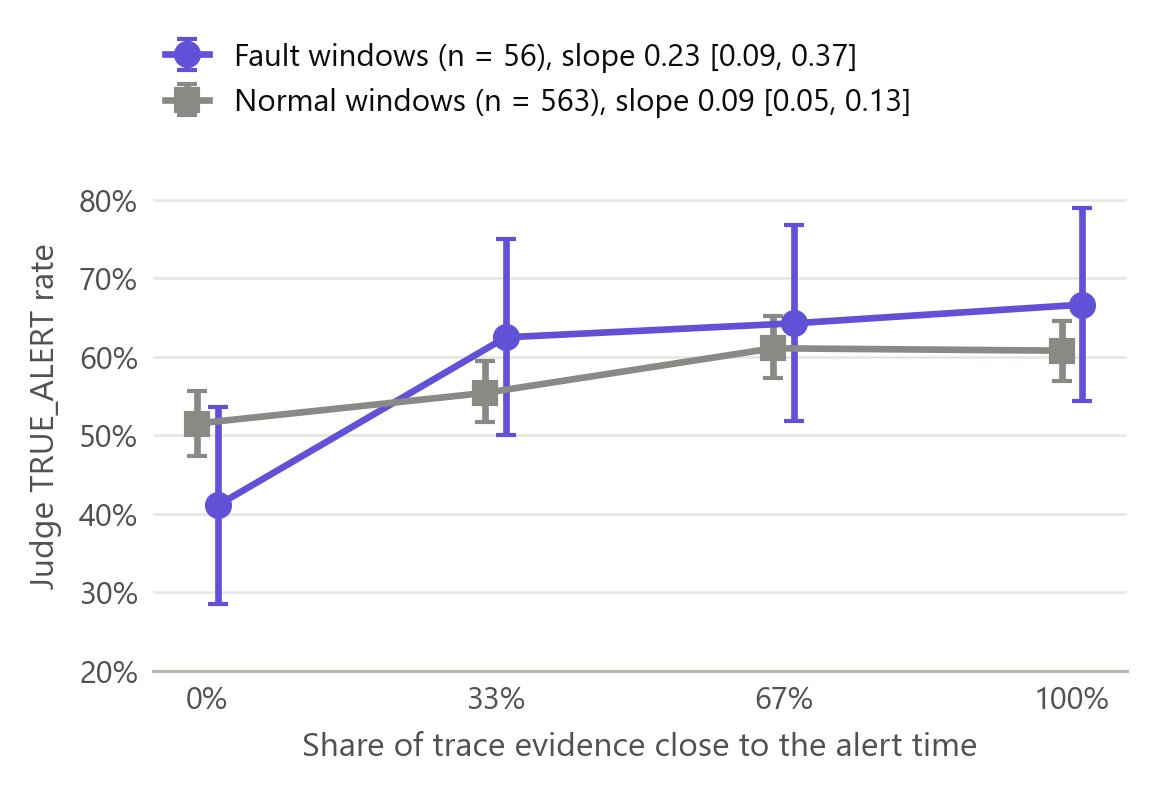
\includegraphics[width=0.92\linewidth]{figures/ch5/h5.4-h1-time-proximity.png}
  \caption[Kết quả thí nghiệm H1 về độ gần thời gian trên tập val]{Thí nghiệm H1 trên tập \splitname{val}: tỷ lệ judge trả \code{TRUE\_ALERT} tăng đơn điệu theo tỷ lệ bằng chứng trace sát thời điểm $t_0$ ở cả cửa sổ bình thường lẫn cửa sổ lỗi (thanh lỗi: CI95 bootstrap).}
  \label{fig:ch5-h1}
\end{figure}

\begin{table}[htbp]
  \centering
  \caption[Tỷ lệ TRUE\_ALERT thô theo điều kiện can thiệp H1 trên tập val]{Tỷ lệ phán quyết \code{TRUE\_ALERT} thô dưới các điều kiện can thiệp ngữ cảnh trong thí nghiệm H1 trên tập \splitname{val}.}
  \label{tab:ch5-h1}
  \scriptsize
  \renewcommand{\arraystretch}{1.15}
  \begin{tabularx}{\linewidth}{@{}l Y c c@{}}
    \toprule
    \textbf{Điều kiện} & \textbf{Mô tả can thiệp ngữ cảnh} & \textbf{Cửa sổ bình thường [CI95]} & \textbf{Cửa sổ lỗi [CI95]} \\
    \midrule
    \code{ref} & Ngữ cảnh C1 tham chiếu & 0,515 [0,486; 0,543] & 0,505 [0,404; 0,596] \\
    \code{time\_0} / \code{33} / \code{67} & Tỷ lệ trace sát $t_0$ tăng dần & 0,515 / 0,554 / 0,611 & 0,411 / 0,625 / 0,643 \\
    \code{near\_trace} & Chỉ đưa trace span của $s_0$ sát $t_0$ & 0,608 [0,570; 0,646] & 0,667 [0,544; 0,789] \\
    \code{near\_log} & Chỉ đưa log của $s_0$ sát $t_0$ & 0,181 [0,146; 0,215] & 0,211 [0,105; 0,316] \\
    \code{neighbor\_trace} & Chỉ đưa trace span từ service lân cận & 0,277 [0,243; 0,314] & 0,386 [0,263; 0,509] \\
    \bottomrule
  \end{tabularx}
\end{table}

\textbf{H1 được giữ một phần trên tập \splitname{val} (không chạy lại trên \splitname{test}).} Thứ tự liệt kê bằng chứng không tạo khác biệt đo được và điểm hiển thị chỉ có tác động nhỏ ($+0{,}020$, $p = 0{,}062$). Ngược lại, hai yếu tố tác động mạnh nhất là \emph{độ gần thời gian} (độ dốc dương ở cả hai nhãn: $+0{,}094$ $[+0{,}050;\, +0{,}134]$ trên bình thường và $+0{,}230$ $[+0{,}086;\, +0{,}370]$ trên lỗi) và \emph{loại bằng chứng} (trace của chính $s_0$ kích hoạt \code{TRUE\_ALERT} tới $60{,}8\%$ trên cửa sổ bình thường, gấp hơn ba lần so với log cục bộ $18{,}1\%$ và hơn gấp đôi trace lân cận $27{,}7\%$). Điểm quan trọng về mặt phương pháp: vì các yếu tố này làm tăng tỷ lệ xác nhận trên cả hai nhãn (độ nhạy chung của judge với bằng chứng trace sát $t_0$), H1 không cung cấp đặc trưng hồ sơ bằng chứng nào phân tách sạch cửa sổ bình thường khỏi cửa sổ lỗi cho C2 — đây là cơ sở trực tiếp dẫn đến việc chuyển trục thiết kế sang neo bằng chứng bất thường C3.

\subsection{Chọn cấu hình \CTAV{} (C3) và loại bỏ C2, C4 trên \splitname{val}}
\label{sec:ch5-val-ctav}

Áp dụng hàm thuần chính sách lên phán quyết đã lưu cache trên \splitname{val}, Bảng~\ref{tab:ch5-val-h3} đối chiếu cấu hình \CTAV{} chốt (C1 + $\theta_{\text{local}} = 0{,}80$ + C3 dùng ngưỡng nền \splitname{dev} $p_{90}$) với từng phép biến đổi một-thay-đổi-một-lần (đường quét ngưỡng $\theta_{\text{topo}}$ chi tiết nằm ở Phụ lục~D). Trên \splitname{val}, bỏ C3 làm cảnh báo sai tăng gần 12 lần ($51 \to 606$ FP) và F1 tụt $-0{,}074$ $[-0{,}124;\, -0{,}027]$; ngược lại, thêm C2 ($\theta_{\text{topo}} = 0{,}85$) chỉ bớt 2 FP ($\Delta\text{FPR} = -0{,}0003$, CI chạm $0$), còn thêm C4 làm chi phí tăng từ $3{,}28$ lên $5{,}14$ USD do tầng 1 BM25 sinh $261$ FP / $15$ TP và tỷ lệ leo thang cao (\textbf{Phát hiện 9}), trong khi F1 giảm nhẹ ($0{,}188$ so với $0{,}201$).

\begin{table}[htbp]
  \centering
  \caption[So sánh các biến thể H3 quanh CTAV trên tập val]{Kết quả lựa chọn cấu hình \CTAV{} và loại trừ từng thành phần trên tập \splitname{val} ($7.636$ cửa sổ có telemetry, $209$ lỗi).}
  \label{tab:ch5-val-h3}
  \scriptsize
  \renewcommand{\arraystretch}{1.15}
  \setlength{\tabcolsep}{3pt}
  \begin{tabularx}{\linewidth}{@{}Y r r r r c r r@{}}
    \toprule
    \textbf{Biến thể trên \splitname{val}} & \textbf{TP} & \textbf{FP} & \textbf{Prec.} & \textbf{Recall} & \textbf{F1 [CI95]} & \textbf{FPR} & \textbf{USD} \\
    \midrule
    \textbf{\CTAV{}} (chốt: C1 + $\theta = 0{,}80$ + C3 \splitname{dev} $p_{90}$) & 29 & 51 & 0,363 & 0,139 & 0,201 [0,138; 0,264] & 0,0069 & 3,28 \\
    + C2 ($\theta_{\text{topo}} = 0{,}85$) & 29 & 49 & 0,372 & 0,139 & 0,202 [0,139; 0,265] & 0,0066 & 3,28 \\
    Bỏ C3 (\code{no\_c3} = C1) & 55 & 606 & 0,083 & 0,263 & 0,126 [0,095; 0,156] & 0,0816 & 3,28 \\
    + C4 (định tuyến hai tầng) & 31 & 90 & 0,256 & 0,148 & 0,188 [0,130; 0,247] & 0,0121 & 5,14 \\
    C3 ngưỡng trượt 60 phút & 34 & 255 & 0,118 & 0,163 & 0,137 [0,097; 0,179] & 0,0343 & 3,28 \\
    \bottomrule
  \end{tabularx}
\end{table}

Dù \CTAV{} đạt F1 sơ bộ cao nhất trên \splitname{val} ($0{,}201$ so với $0{,}103$ của BM25, $\Delta\text{F1} = +0{,}098$ $[+0{,}046;\, +0{,}149]$) và giảm FPR gấp $8$ lần so với BM25, hai giới hạn quan trọng đã được ghi nhận ngay trước khi khóa cấu hình: (i) Recall của \CTAV{} giảm xuống $0{,}139$ so với $0{,}263$ của C1 ($\Delta\text{Recall} = -0{,}124$, \textbf{Phát hiện 10}), và (ii) ngưỡng nền \splitname{dev} $p_{90}$ chỉ phủ $31{,}8\%$--$33{,}2\%$ span trên \splitname{val} do $15$ service không có cửa sổ bình thường trong \splitname{dev} (\textbf{Phát hiện 8}), khiến ưu thế của ngưỡng tĩnh \splitname{dev} một phần đến từ việc im lặng có cấu trúc ở nhóm service thiếu ngưỡng (\textbf{Phát hiện 11}). Theo quy tắc lựa chọn đã ghi trước, cấu hình chốt giữ \splitname{dev} $p_{90}$ và đưa biến thể ngưỡng trượt 60 phút (\code{c3\_rolling\_baseline}, phủ $93\%$ span) vào diện theo dõi bắt buộc trong H3 trên \splitname{test}.

\subsection{Khảo sát cổng cứu cảnh báo C5 trên \splitname{val}}
\label{sec:ch5-c5}

Trên tập \splitname{val}, hệ thống tính ngoại tuyến $147$ điểm lưới $(\eta_1, \eta_2, \eta_3, \tau)$ của C5 (\code{Rescue Score}) với tập cảnh báo kích hoạt nhân quả $A$ là $80$ cảnh báo của \CTAV{} trong cửa sổ $300\,\text{s}$ và chấm một lần $1.459$ cửa sổ được cứu ($1{,}03$ USD theo token; đường quét $\tau$ nằm ở Phụ lục~D). Điểm tối ưu trên \splitname{val} là $\eta = (0;\, 0{,}4;\, 0{,}6)$ và $\tau = 0{,}8$ (thành phần log lỗi $\Lambda_{\text{log}}$ không đóng góp vì bằng $0$ ở hầu hết cửa sổ). Bảng~\ref{tab:ch5-val-c5} cho thấy C5 tốn thêm $52$ lượt gọi LLM nhưng chỉ thu thêm $2$ TP trong khi tăng $16$ FP ($\Delta\text{F1} = +0{,}001$ $[-0{,}014;\, +0{,}022]$, $\Delta\text{FPR} = +0{,}0022$ $[+0{,}0011;\, +0{,}0034]$, McNemar $p = 0{,}0013$). Nguyên nhân là nút thắt nằm ở chính bộ thẩm định LLM ($16/21$ cửa sổ lỗi được cứu bị C1 trả \code{FALSE\_POSITIVE}, $3$ ca khác bị C3 hạ, \textbf{Phát hiện 12}). Vì vậy, C5 bị loại khỏi cấu hình \CTAV{} chính và chỉ giữ đúng một điểm cố định cho phép kiểm tra ablation trên \splitname{test}.

\begin{table}[htbp]
  \centering
  \caption[Kết quả cổng cứu cảnh báo C5 trên tập val]{Hiệu quả bổ sung cổng Rescue (C5) tại điểm chọn $\eta = (0;\, 0{,}4;\, 0{,}6)$, $\tau = 0{,}8$ trên tập \splitname{val} ($7.636$ cửa sổ có telemetry, $209$ lỗi).}
  \label{tab:ch5-val-c5}
  \scriptsize
  \renewcommand{\arraystretch}{1.15}
  \begin{tabularx}{\linewidth}{@{}Y r r r r c r@{}}
    \toprule
    \textbf{Cấu hình trên \splitname{val}} & \textbf{+ Lần gọi} & \textbf{TP} & \textbf{FP} & \textbf{Recall} & \textbf{F1 [CI95]} & \textbf{FPR} \\
    \midrule
    \CTAV{} (tắt C5) & 0 & 29 & 51 & 0,139 & 0,201 [0,138; 0,264] & 0,0069 \\
    \CTAV{} + C5 & +52 & 31 & 67 & 0,148 & 0,202 [0,143; 0,261] & 0,0090 \\
    \bottomrule
  \end{tabularx}
\end{table}

% -----------------------------------------------------------------------------
\section{Kết quả kiểm định trên tập \splitname{test} (G-test)}
\label{sec:ch5-test}

Sau khi đăng ký toàn bộ giả thuyết và khóa cấu hình tại commit \code{be2b985}, tập \splitname{test} ($46.849$ cửa sổ, trong đó $11.985$ cửa sổ có telemetry và $346$ cửa sổ lỗi) được chạy đúng một lần mà không điều chỉnh bất kỳ tham số nào.

\subsection{Giao thức G-test và tổng hợp các lượt chạy}
\label{sec:ch5-test-protocol}

Tất cả cấu hình chạy trên \splitname{test} đều là bản sao nguyên vẹn từ cấu hình \splitname{val}, chỉ thay đổi tên split và mã lượt chạy \code{run\_id}. Bộ thẩm định chấm toàn bộ $13.699$ candidate của \splitname{test} để đảm bảo số liệu đầy đủ cho cả tập chấm chính lẫn tập phụ. Bảng~\ref{tab:ch5-test-runs} tổng hợp toàn bộ các lượt chạy trên \splitname{test}: tổng cộng phát sinh $21.094$ lượt gọi API mới ($15{,}85$ USD theo token) với $0$ lỗi judge. C1 chỉ cần gọi $3.299$ lượt API mới vì $10.400$ candidate không có bằng chứng dùng lại chính xác câu trả lời đã lưu cache của BM25; tương tự, lượt chạy \code{h0\_test\_norag\_v2} tái sử dụng các câu trả lời đã lưu từ cache mà không ghi đè thư mục cũ.

\begin{table}[htbp]
  \centering
  \caption[Danh sách các lượt chạy kiểm định trên tập test]{Tổng hợp các lượt chạy chính thức của cổng G-test trên tập \splitname{test} ($46.849$ cửa sổ, $13.699$ candidate).}
  \label{tab:ch5-test-runs}
  \scriptsize
  \renewcommand{\arraystretch}{1.15}
  \setlength{\tabcolsep}{3pt}
  \begin{tabularx}{\linewidth}{@{}l Y r r r r@{}}
    \toprule
    \textbf{Mã lượt chạy (\code{run\_id})} & \textbf{Nội dung} & \textbf{Lượt gọi LLM} & \textbf{API mới} & \textbf{Lỗi} & \textbf{USD mới} \\
    \midrule
    \code{m8\_test\_detector\_count\_v1} & Chỉ detector (đếm candidate) & 0 & 0 & -- & 0,00 \\
    \code{h0\_test\_bm25\_v1} & BM25 + judge & 13.699 & 13.699 & 0 & 8,87 \\
    \code{h0\_test\_c1\_k0\_v1} & C1 + judge & 13.699 & 3.299 & 0 & 4,71 \\
    \code{h0\_test\_norag\_v2} & LLM-không-RAG (kế tiếp cache \code{\_v1}) & 13.699 & 3.287 & 0 & 1,10 \\
    \code{h0\_test\_*\_b120\_v1} & Ba lượt ngân sách 120 lần gọi & $3 \times 120$ & 0 & 0 & 0,00 \\
    \code{ctav\_final\_test\_v1} & Replay \CTAV{} + 4 nhánh ablation & 0 (replay) & 0 & -- & 0,00 \\
    \code{m8\_rescue\_test\_c1\_v1} & C5 một điểm (cửa sổ được cứu) & 61 & 61 & 0 & 0,09 \\
    \code{h0\_test\_*\_rep\{1,2\}\_v1} & Đo phương sai judge ($4 \times 200$ cửa sổ) & 800 & 748 & 0 & 1,08 \\
    \midrule
    \textbf{Tổng G-test} & & & \textbf{21.094} & \textbf{0} & \textbf{15,85} \\
    \bottomrule
  \end{tabularx}
\end{table}

\subsection{Hành vi bộ phát hiện trên \splitname{test} và độ lệch giữa các split}
\label{sec:ch5-test-shift}

Trước khi đọc các chỉ số so sánh, cần nắm rõ phân bố ứng viên đầu vào đã dịch chuyển giữa các split dù ngưỡng Isolation Forest ($0{,}85$) không đổi (Hình~\ref{fig:ch5-shift} và Bảng~\ref{tab:ch5-shift}). Theo cách chuẩn hóa phân vị trên \splitname{dev}, tỷ lệ candidate trên \splitname{dev} đúng bằng $15{,}0\%$; sang \splitname{val} tăng lên $19{,}6\%$ và sang \splitname{test} đạt $29{,}2\%$ ($13.699 / 46.849$ cửa sổ).

\begin{figure}[htbp]
  \centering
  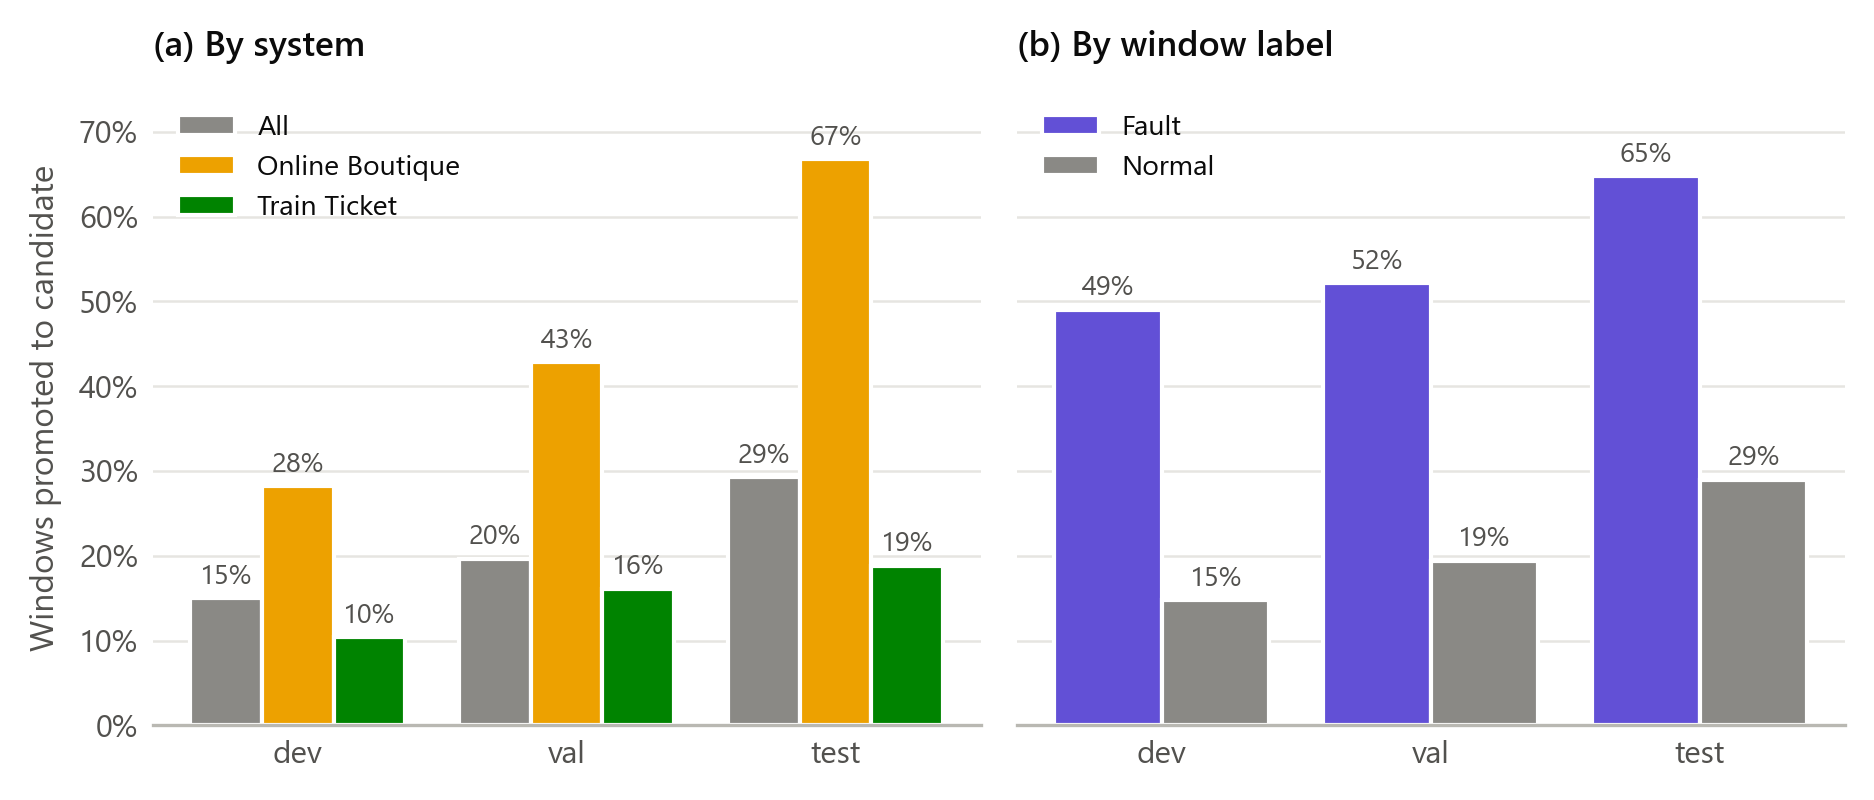
\includegraphics[width=0.92\linewidth]{figures/ch5/h5.8-candidate-rate-by-split.png}
  \caption[Tỷ lệ candidate của detector trên ba split dev, val và test]{Tỷ lệ cửa sổ trở thành candidate ($\text{score}_{\text{IF}} \ge 0{,}85$) trên \splitname{dev}, \splitname{val}, \splitname{test}: (a)~theo hệ thống và (b)~theo nhãn cửa sổ.}
  \label{fig:ch5-shift}
\end{figure}

\begin{table}[htbp]
  \centering
  \caption[So sánh hành vi bộ phát hiện đã đóng băng trên ba split]{Thống kê bộ phát hiện Isolation Forest (ngưỡng $0{,}85$, huấn luyện trên \splitname{dev}) qua ba split \splitname{dev}, \splitname{val} và \splitname{test}.}
  \label{tab:ch5-shift}
  \scriptsize
  \renewcommand{\arraystretch}{1.15}
  \begin{tabularx}{\linewidth}{@{}Y r r r@{}}
    \toprule
    \textbf{Chỉ tiêu} & \textbf{\splitname{dev}} & \textbf{\splitname{val}} & \textbf{\splitname{test}} \\
    \midrule
    Tổng cửa sổ & 19.316 & 28.898 & 46.849 \\
    Số candidate (tỷ lệ) & 2.898 (15,0\%) & 5.677 (19,6\%) & 13.699 (29,2\%) \\
    Điểm bất thường trung vị / p90 & 0,500 / 0,900 & 0,549 / 0,910 & 0,588 / 0,953 \\
    Recall detector-only & 73 / 149 (0,490) & 109 / 209 (0,522) & 224 / 346 (0,647) \\
    FPR detector-only (có telemetry) & 825 / 4.881 (0,1693) & 1.640 / 7.427 (0,2208) & 3.435 / 11.639 (0,2951) \\
    OnlineBoutique: tỷ trọng split; tỷ lệ candidate & 25,8\%; 28,2\% & 13,2\%; 42,8\% & 21,8\%; 66,8\% \\
    TrainTicket: tỷ lệ candidate & 10,4\% & 16,1\% & 18,8\% \\
    Số service ``luôn bật'' ($\ge 90\%$ candidate) & 2 & 3 & 5 \\
    \bottomrule
  \end{tabularx}
\end{table}

Độ lệch này không xuất phát từ một ngày đơn lẻ mà đến từ thành phần service của từng split khi chia theo lần tiêm lỗi: \splitname{test} có tỷ trọng cửa sổ OnlineBoutique cao hơn \splitname{val} ($21{,}8\%$ so với $13{,}2\%$) với tỷ lệ candidate tới $66{,}8\%$, trong đó năm service gần như luôn vượt ngưỡng (\code{checkoutservice}, \code{currencyservice}, \code{frontend}, \code{productcatalogservice}, \code{ts-ui-dashboard}) tạo ra $6.407$ candidate ($47\%$ toàn bộ \splitname{test}; riêng \code{frontend} không xuất hiện ở \splitname{val}). Ba hệ quả trực tiếp cần lưu ý khi đọc kết quả phía sau: (i) bộ phát hiện trên \splitname{test} có cả Recall ($0{,}647$) lẫn FPR ($0{,}2951$) cao hơn \splitname{val}; (ii) mốc $4.000$ lần gọi trên đường ngân sách chỉ phủ $29\%$ candidate của \splitname{test} và nằm trọn trong ngày đầu tiên của OnlineBoutique; và (iii) chi phí chấm toàn bộ \splitname{test} cao gấp $2{,}4$ lần \splitname{val}.

\subsection{Bức tranh tổng quan các phương pháp trên \splitname{test}}
\label{sec:ch5-test-overview}

Bảng~\ref{tab:ch5-test-overview} và Hình~\ref{fig:ch5-operating} đặt năm phương pháp trên mặt phẳng Recall--FPR của tập chấm chính (\splitname{test}: $11.985$ cửa sổ có telemetry, $346$ lỗi) cạnh các điểm tham chiếu trên \splitname{val}. Thứ tự trên trục FPR được bảo toàn tuyệt đối giữa hai split: $\text{\CTAV} < \text{BM25} \approx \text{không-RAG} < \text{C1} < \text{detector-only}$. Cụ thể, \CTAV{} đạt FPR thấp nhất toàn bảng ($0{,}0055$, chỉ $64$ cảnh báo sai trên $11.639$ cửa sổ bình thường) và Precision cao nhất ($0{,}179$), nhưng Recall giảm xuống còn $0{,}040$ ($14$ TP) khiến F1 hạ từ $0{,}201$ trên \splitname{val} xuống $0{,}066$ trên \splitname{test}. Ở chiều ngược lại, trên tập phụ gồm mọi cửa sổ ($46.849$ cửa sổ), BM25, C1 và \CTAV{} giữ nguyên số TP/FP nhờ luật \code{require\_evidence}, còn LLM-không-RAG sinh thêm $832$ cảnh báo sai trên vùng không có telemetry (tổng $1.203$ FP, F1 tụt còn $0{,}047$).

\begin{figure}[htbp]
  \centering
  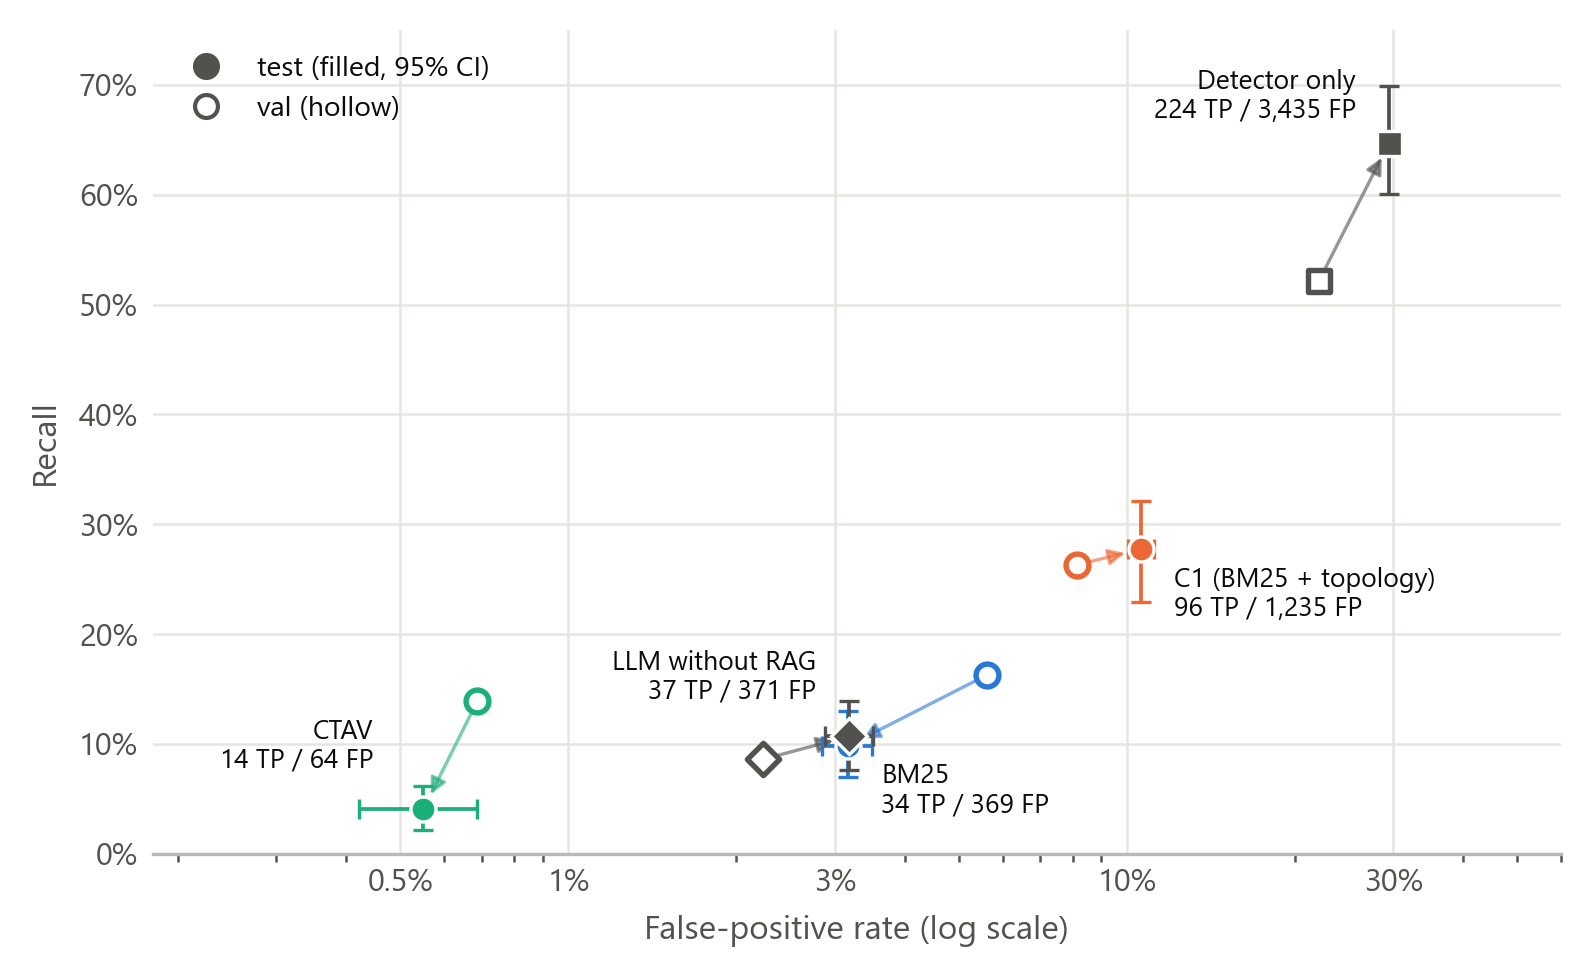
\includegraphics[width=0.92\linewidth]{figures/ch5/h5.9-recall-fpr-operating-points.png}
  \caption[Điểm vận hành Recall--FPR của năm phương pháp trên val và test]{Điểm vận hành Recall--FPR (trục FPR thang log) trên cửa sổ có telemetry của \splitname{val} (điểm rỗng) và \splitname{test} (điểm đặc kèm CI95 và nhãn TP/FP).}
  \label{fig:ch5-operating}
\end{figure}

\begin{table}[htbp]
  \centering
  \caption[So sánh tổng quan năm phương pháp trên test cạnh val]{Hiệu năng năm phương pháp trên \splitname{test} (cửa sổ có telemetry: $11.985$ cửa sổ, $346$ lỗi) cạnh tham chiếu \splitname{val} ($7.636$ cửa sổ, $209$ lỗi).}
  \label{tab:ch5-test-overview}
  \scriptsize
  \renewcommand{\arraystretch}{1.15}
  \setlength{\tabcolsep}{2.5pt}
  \begin{tabularx}{\linewidth}{@{}Y r r r c c c r@{}}
    \toprule
    \textbf{Phương pháp} & \textbf{TP} & \textbf{FP} & \textbf{Prec.} & \textbf{Recall [CI95]} & \textbf{F1 [CI95]} & \textbf{FPR [CI95]} & \textbf{\splitname{val} F1} \\
    \midrule
    Detector-only & 224 & 3.435 & 0,061 & 0,647 [0,601; 0,699] & 0,112 [0,100; 0,126] & 0,2951 [0,2870; 0,3036] & 0,111 \\
    LLM-không-RAG & 37 & 371 & 0,091 & 0,107 [0,077; 0,139] & 0,098 [0,071; 0,126] & 0,0319 [0,0288; 0,0351] & 0,092 \\
    BM25 & 34 & 369 & 0,084 & 0,098 [0,070; 0,130] & 0,091 [0,064; 0,119] & 0,0317 [0,0285; 0,0350] & 0,103 \\
    C1 ($k_{\text{graph}} = 0$) & 96 & 1.235 & 0,072 & 0,277 [0,230; 0,321] & 0,114 [0,093; 0,135] & 0,1061 [0,1007; 0,1118] & 0,126 \\
    \textbf{\CTAV{}} (\splitname{dev} $p_{90}$) & \textbf{14} & \textbf{64} & \textbf{0,179} & \textbf{0,040 [0,022; 0,061]} & \textbf{0,066 [0,036; 0,100]} & \textbf{0,0055 [0,0042; 0,0069]} & 0,201 \\
    \midrule
    \emph{Đối chứng H3:} C3-trượt & 47 & 391 & 0,107 & 0,136 [0,101; 0,172] & 0,120 [0,090; 0,151] & 0,0336 [0,0304; 0,0369] & 0,137 \\
    \bottomrule
  \end{tabularx}
\end{table}

\subsection{Kiểm định H0: topology chưa hiệu chỉnh tăng recall và FPR}
\label{sec:ch5-test-h0}

Giả thuyết H0 kiểm tra liệu truy xuất nhận biết topology chưa hiệu chỉnh (C1) có làm tăng đồng thời Recall và FPR so với BM25 trên tập \splitname{test} hay không. Theo bản đăng ký, H0 chỉ được chấp nhận khi đạt cả bốn vế: CI95 của $\Delta\text{Recall}(\text{C1}-\text{BM25})$ có cận dưới $> 0$, CI95 của $\Delta\text{FPR}(\text{C1}-\text{BM25})$ có cận dưới $> 0$, và kiểm định McNemar trên cả cửa sổ lỗi lẫn cửa sổ bình thường đều cho $p < 0{,}05$ (Bảng~\ref{tab:ch5-test-h0}).

\begin{table}[htbp]
  \centering
  \caption[Kiểm định giả thuyết H0 trên tập test]{Kết quả kiểm định H0 (C1 $-$ BM25) trên tập \splitname{test} ($11.985$ cửa sổ có telemetry, $346$ lỗi) cạnh tham chiếu \splitname{val}.}
  \label{tab:ch5-test-h0}
  \scriptsize
  \renewcommand{\arraystretch}{1.15}
  \setlength{\tabcolsep}{3pt}
  \begin{tabularx}{\linewidth}{@{}Y >{\raggedright\arraybackslash}p{4.6cm} l >{\raggedright\arraybackslash}p{3.1cm}@{}}
    \toprule
    \textbf{Vế tiêu chí H0} & \textbf{Số đo trên \splitname{test}} & \textbf{Kết quả} & \textbf{\splitname{val} (tham chiếu)} \\
    \midrule
    CI95 $\Delta\text{Recall}(\text{C1}-\text{BM25})$ cận dưới $> 0$ & $+0{,}179$ $[+0{,}138;\, +0{,}226]$ & \textbf{Đạt} & $+0{,}100$ $[+0{,}052;\, +0{,}155]$ \\
    CI95 $\Delta\text{FPR}(\text{C1}-\text{BM25})$ cận dưới $> 0$ & $+0{,}0744$ $[+0{,}0694;\, +0{,}0798]$ & \textbf{Đạt} & $+0{,}0254$ $[+0{,}0204;\, +0{,}0306]$ \\
    McNemar cửa sổ lỗi, $p < 0{,}05$ & $p < 0{,}001$ (C1 đúng/BM25 sai: 65; ngược lại: 3) & \textbf{Đạt} & $p < 0{,}001$ (28; 7) \\
    McNemar cửa sổ bình thường, $p < 0{,}05$ & $p < 0{,}001$ (BM25 đúng/C1 sai: 966; ngược lại: 100) & \textbf{Đạt} & $p < 0{,}001$ (276; 87) \\
    \emph{Phụ:} $\Delta\text{F1}$ (ngoài tiêu chí) & $+0{,}024$ $[-0{,}001;\, +0{,}052]$ & -- & $+0{,}023$ $[-0{,}004;\, +0{,}052]$ \\
    \bottomrule
  \end{tabularx}
\end{table}

\textbf{H0 được chấp nhận trên tập \splitname{test} (đạt 4/4 vế).} So với BM25, C1 bắt thêm $62$ cửa sổ lỗi ($96$ so với $34$ TP; có $65$ cửa sổ lỗi C1 bắt đúng mà BM25 bỏ sót, chiều ngược lại chỉ $3$) nhưng đồng thời tạo thêm $866$ cảnh báo sai ($1.235$ so với $369$ FP; FPR tăng gấp $3{,}3$ lần). So với \splitname{val}, hiện tượng lặp lại với biên độ lớn hơn ở cả hai chiều, trong khi CI95 của $\Delta\text{F1}$ tiếp tục chứa $0$ ($[-0{,}001;\, +0{,}052]$). Lưu ý rằng H0 kiểm định hiện tượng đầu ra; cơ chế gây nhiễu đã được khảo sát ở H1 trên \splitname{val} và không chạy lại trên \splitname{test}.

\subsection{Kiểm định H2: \CTAV{} so với BM25 và C1 (giả thuyết chính)}
\label{sec:ch5-test-h2}

Giả thuyết chính H2 kiểm tra liệu cấu hình \CTAV{} đã đóng băng có đạt đồng thời ba vế tiêu chí đã đăng ký hay không: (i)~CI95 của $\Delta\text{F1}(\text{\CTAV}-\text{BM25})$ có cận dưới $> 0$ và McNemar $p < 0{,}05$; (ii)~CI95 của $\Delta\text{FPR}(\text{\CTAV}-\text{BM25})$ không có cận dưới $> 0$; và (iii)~ước lượng điểm $\Delta\text{Recall}(\text{\CTAV}-\text{C1}) \ge -0{,}05$. Hình~\ref{fig:ch5-forest} trực quan hóa toàn bộ các hiệu ghép cặp và CI95 trên cả hai split, còn Bảng~\ref{tab:ch5-test-h2} đối chiếu từng vế tiêu chí của H2.

\begin{figure}[htbp]
  \centering
  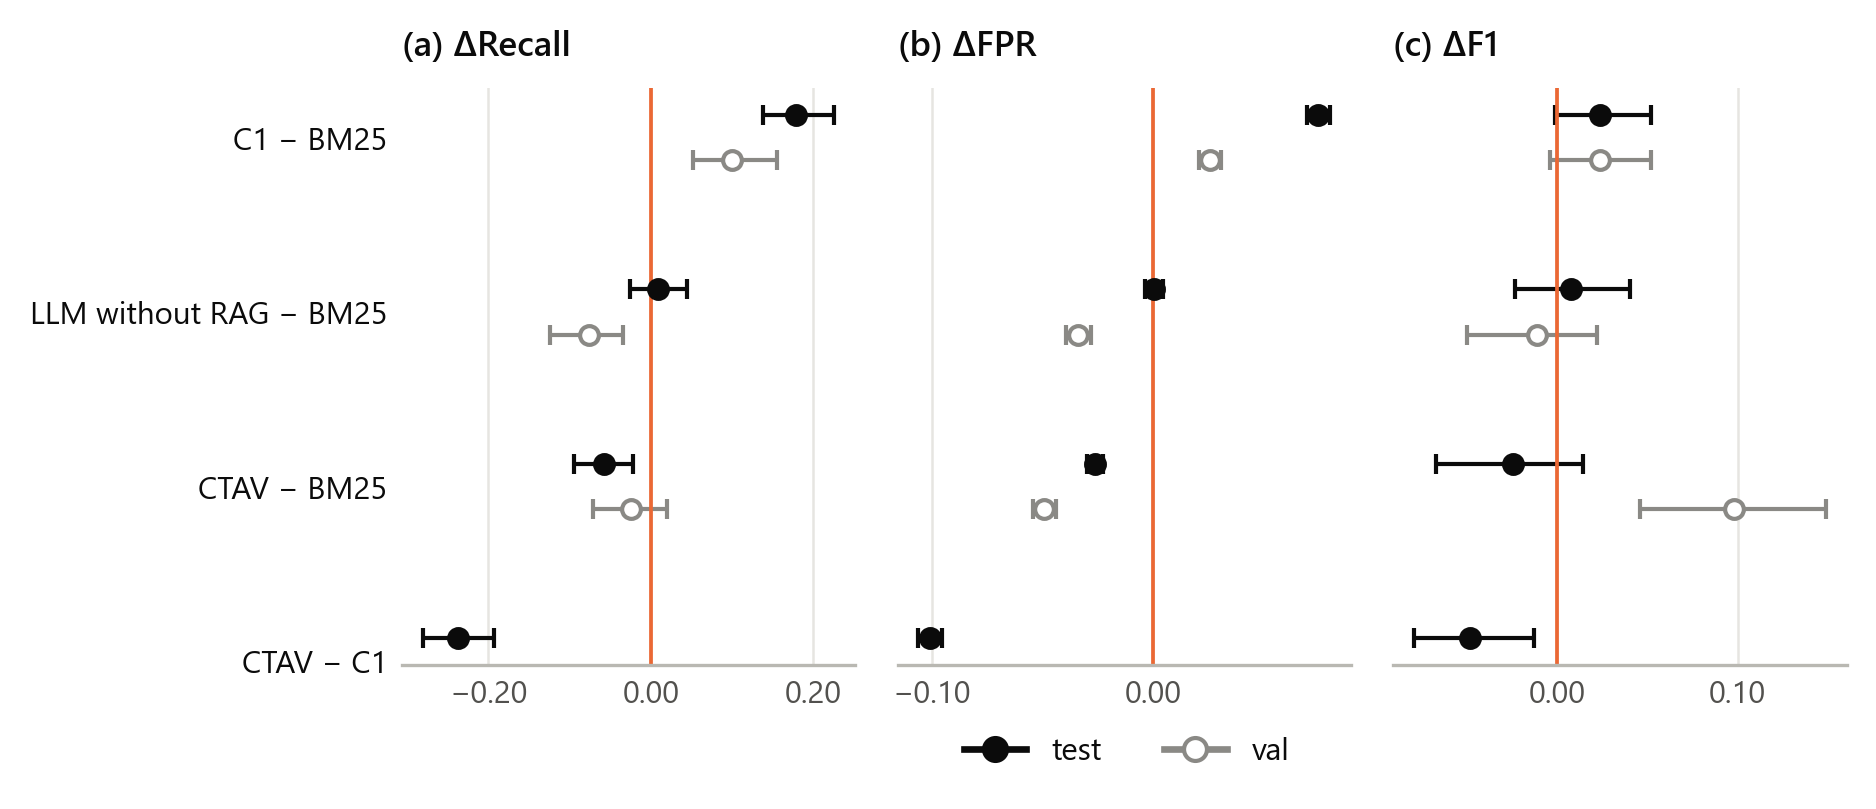
\includegraphics[width=\linewidth]{figures/ch5/h5.10-paired-differences-ci.png}
  \caption[Hiệu ghép cặp và khoảng tin cậy CI95 của các phương pháp]{Hiệu ghép cặp $\Delta\text{Recall}$, $\Delta\text{FPR}$ và $\Delta\text{F1}$ kèm CI95 bootstrap trên \splitname{test} (điểm đặc) và \splitname{val} (điểm rỗng); vạch dọc tại $0$ giúp nhận diện ngay vế có ý nghĩa thống kê.}
  \label{fig:ch5-forest}
\end{figure}

\begin{table}[htbp]
  \centering
  \caption[Kiểm định giả thuyết chính H2 trên tập test]{Kết quả kiểm định H2 trên tập \splitname{test} ($11.985$ cửa sổ có telemetry, $346$ lỗi) cạnh tham chiếu \splitname{val}.}
  \label{tab:ch5-test-h2}
  \scriptsize
  \renewcommand{\arraystretch}{1.15}
  \setlength{\tabcolsep}{3pt}
  \begin{tabularx}{\linewidth}{@{}Y l >{\raggedright\arraybackslash}p{4.1cm} l >{\raggedright\arraybackslash}p{2.6cm}@{}}
    \toprule
    \textbf{Vế tiêu chí H2} & \textbf{So sánh} & \textbf{Số đo trên \splitname{test}} & \textbf{Kết quả} & \textbf{\splitname{val} (sơ bộ)} \\
    \midrule
    (i) CI95 $\Delta\text{F1}$ cận dưới $> 0$ \& McNemar $p < 0{,}05$ & \CTAV{} $-$ BM25 & $-0{,}025$ $[-0{,}067;\, +0{,}014]$; $p < 0{,}001$ & \textbf{Không đạt} & $+0{,}098$ $[+0{,}046;\, +0{,}149]$ \\
    (ii) CI95 $\Delta\text{FPR}$ không có cận dưới $> 0$ & \CTAV{} $-$ BM25 & $-0{,}0262$ $[-0{,}0297;\, -0{,}0229]$ & \textbf{Đạt} & $-0{,}0493$ $[-0{,}0545;\, -0{,}0439]$ \\
    (iii) $\Delta\text{Recall} \ge -0{,}05$ (ước lượng điểm) & \CTAV{} $-$ C1 & $-0{,}237$ $[-0{,}281;\, -0{,}193]$ & \textbf{Không đạt} & $-0{,}124$ (không đạt) \\
    \emph{Phụ:} $\Delta\text{Precision}$ & \CTAV{} $-$ BM25 & $+0{,}095$ $[+0{,}014;\, +0{,}186]$ & -- & $+0{,}279$ \\
    \emph{Phụ:} $\Delta\text{Recall}$ & \CTAV{} $-$ BM25 & $-0{,}058$ $[-0{,}095;\, -0{,}022]$ & -- & $-0{,}024$ \\
    \emph{Phụ:} $\Delta\text{F1}$ & \CTAV{} $-$ C1 & $-0{,}048$ $[-0{,}079;\, -0{,}013]$ & -- & $+0{,}074$ \\
    \emph{Phụ:} $\Delta\text{F1}$ & \CTAV{} $-$ không-RAG & $-0{,}032$ $[-0{,}075;\, +0{,}008]$ & -- & $+0{,}109$ \\
    \bottomrule
  \end{tabularx}
\end{table}

\textbf{H2 không được chấp nhận trên tập \splitname{test}.} Theo số đếm trên $11.985$ cửa sổ có telemetry, vế (ii) đạt rất rõ rệt: \CTAV{} loại $305$ cảnh báo sai so với BM25 ($369 \to 64$ FP, giảm $5{,}8$ lần) và loại $1.171$ cảnh báo sai so với C1 ($1.235 \to 64$ FP, giảm $94{,}8\%$), nâng Precision hơn gấp đôi so với BM25 ($0{,}179$ so với $0{,}084$, $\Delta\text{Precision} = +0{,}095$ $[+0{,}014;\, +0{,}186]$). Tuy nhiên, bộ lọc C3 dùng ngưỡng tĩnh \splitname{dev} đồng thời làm rơi $82 / 96$ TP của C1 (còn $14$ TP, thấp hơn $34$ TP của BM25; McNemar riêng trên cửa sổ lỗi $p = 0{,}004$), khiến cả vế (iii) ($\Delta\text{Recall} = -0{,}237 < -0{,}05$) lẫn vế (i) ($\Delta\text{F1} = -0{,}025$ $[-0{,}067;\, +0{,}014]$, CI chứa $0$) đều không đạt. So với \splitname{val}, mức giảm FPR nhất quán ($0{,}0069 \to 0{,}0055$), nhưng mức hụt recall so với C1 tăng gần gấp đôi ($-0{,}124 \to -0{,}237$), chuyển kết luận từ ``đạt một phần'' trên \splitname{val} thành ``không được chấp nhận'' trên \splitname{test}. Nguyên nhân cốt lõi (độ phủ ngưỡng nền \splitname{dev}) được định lượng chi tiết ở Mục~\ref{sec:ch5-finding11}.

\subsection{Kiểm định H3: đóng góp của từng thành phần}
\label{sec:ch5-test-h3}

Giả thuyết H3 kiểm định vai trò của từng thành phần quanh \CTAV{} bằng phương pháp một-thay-đổi-một-lần theo ba tiêu chí đăng ký (Bảng~\ref{tab:ch5-test-h3}): bỏ C3 phải làm CI95 của $\Delta\text{Precision}$ có cận trên $< 0$; thêm lại C2 ($\theta_{\text{topo}} = 0{,}85$) xác nhận quyết định loại nếu CI95 $\Delta\text{FPR}$ chứa $0$ hoặc $> 0$; và thêm lại C4 xác nhận quyết định loại nếu chi phí tăng mà CI95 $\Delta\text{F1}$ không có cận dưới $> 0$. Hai biến thể C3-trượt và C5 một điểm được báo mô tả kèm theo.

\begin{table}[htbp]
  \centering
  \caption[Kiểm định giả thuyết H3 trên tập test]{Kết quả kiểm định H3 theo từng thành phần trên tập \splitname{test} ($11.985$ cửa sổ có telemetry, $346$ lỗi).}
  \label{tab:ch5-test-h3}
  \scriptsize
  \renewcommand{\arraystretch}{1.15}
  \setlength{\tabcolsep}{3pt}
  \begin{tabularx}{\linewidth}{@{}l Y >{\raggedright\arraybackslash}p{4.2cm} l@{}}
    \toprule
    \textbf{Thành phần} & \textbf{Tiêu chí đã đăng ký} & \textbf{Số đo trên \splitname{test}} & \textbf{Kết quả} \\
    \midrule
    C3 (đang dùng) & Bỏ C3 $\Rightarrow$ CI95 $\Delta\text{Precision}$ cận trên $< 0$ & $-0{,}107$ $[-0{,}197;\, -0{,}030]$ & \textbf{Đạt} (đóng góp) \\
    C2 (đã loại) & Thêm C2: CI95 $\Delta\text{FPR}$ chứa $0$ hoặc $> 0$ & $+0{,}0000$ $[+0{,}0000;\, +0{,}0000]$ & \textbf{Đạt} (xác nhận loại) \\
    C4 (đã loại) & Thêm C4: chi phí tăng \& CI95 $\Delta\text{F1}$ không có cận dưới $> 0$ & $-0{,}001$ $[-0{,}001;\, +0{,}000]$; $13{,}56$ vs $8{,}16$ USD & \textbf{Đạt} (xác nhận loại) \\
    C3-trượt & Báo mô tả $\Delta\text{F1}$, $\Delta\text{FPR}$, $\Delta\text{Recall}$ & $\Delta\text{F1} = +0{,}054$ $[+0{,}017;\, +0{,}091]$; $\Delta\text{FPR} = +0{,}0281$; $\Delta\text{Recall} = +0{,}095$ & Mô tả \\
    C5 một điểm & Báo mô tả $\Delta\text{Recall}$, $\Delta\text{FPR}$, +lần gọi & $\Delta\text{Recall} = +0{,}000$; $\Delta\text{FPR} = +0{,}0001$; $+61$ lần gọi & Mô tả \\
    \bottomrule
  \end{tabularx}
\end{table}

\textbf{H3 được chấp nhận trên tập \splitname{test} (đạt cả ba tiêu chí thành phần).} Khi bỏ C3, báo động sai nhảy từ $64$ lên $1.235$ FP làm Precision tụt $0{,}107$; thêm lại C2 không thay đổi một phán quyết cuối nào ($0$ TP, $0$ FP thay đổi vì toàn bộ $54$ ca bị C2 hạ đều đã bị C3 hạ trước đó); còn thêm lại C4 tiêu tốn thêm $3.286$ lượt gọi LLM ($13{,}56$ so với $8{,}16$ USD quy đổi cả cache) và thêm $4$ FP mà không thêm TP nào. Đối chiếu với \splitname{val}, cả ba quyết định giữ C3 và loại C2, C4 đều nhất quán hoàn toàn; điểm đảo chiều duy nhất là biến thể \code{C3-trượt} tăng thêm $33$ TP ($14 \to 47$ TP) và nâng F1 thêm $+0{,}054$ $[+0{,}017;\, +0{,}091]$ lên $0{,}120$, khẳng định sự khác biệt nằm ở cách ước lượng ngưỡng nền.

\subsection{Kiểm định H4: hiệu quả ở ngân sách nhỏ 120 lần gọi}
\label{sec:ch5-h4}

Giả thuyết H4 kiểm tra điều kiện ngân sách hạn hẹp ở $120$ lượt gọi LLM đầu tiên theo thứ tự thời gian, với tiêu chí đăng ký là ước lượng điểm $\text{F1}(\text{\CTAV}) \ge \text{F1}(\text{LLM-không-RAG})$ (Bảng~\ref{tab:ch5-test-h4}).

\begin{table}[htbp]
  \centering
  \caption[Kiểm định giả thuyết H4 ở ngân sách 120 lần gọi trên test]{So sánh bốn phương pháp ở ngân sách 120 lượt gọi LLM đầu tiên trên \splitname{test} ($11.985$ cửa sổ có telemetry, $346$ lỗi) cạnh tham chiếu \splitname{val}.}
  \label{tab:ch5-test-h4}
  \scriptsize
  \renewcommand{\arraystretch}{1.15}
  \begin{tabularx}{\linewidth}{@{}Y r r r r c r@{}}
    \toprule
    \textbf{Phương pháp} & \textbf{TP} & \textbf{FP} & \textbf{Precision} & \textbf{Recall} & \textbf{F1 [CI95] (\splitname{test})} & \textbf{F1 (\splitname{val})} \\
    \midrule
    \textbf{\CTAV{}} & 6 & 0 & 1,000 & 0,017 & \textbf{0,034 [0,011; 0,064]} & 0,028 \\
    LLM-không-RAG & 3 & 3 & 0,500 & 0,009 & 0,017 [0,000; 0,038] & 0,000 \\
    BM25 & 3 & 3 & 0,500 & 0,009 & 0,017 [0,000; 0,038] & 0,016 \\
    C1 & 11 & 23 & 0,324 & 0,032 & 0,058 [0,026; 0,092] & 0,023 \\
    \bottomrule
  \end{tabularx}
\end{table}

\textbf{H4 được chấp nhận trên tập \splitname{test}.} Trong $120$ candidate đầu tiên, \CTAV{} bắt $6$ TP với $0$ FP ($\text{Precision} = 1{,}000$, $\text{F1} = 0{,}034$), gấp đôi số TP của LLM-không-RAG và BM25 (cùng $3$ TP, $3$ FP, $\text{F1} = 0{,}017$), trùng chiều quan sát trên \splitname{val} ($0{,}028$ so với $0{,}000$). Tuy nhiên, cần đọc kèm hai giới hạn: $120$ lượt gọi chỉ bằng $0{,}9\%$ tổng số candidate của \splitname{test} khiến CI95 chồng nhau rộng giữa hai phương pháp, và toàn bộ $120$ candidate đầu thuộc đầu ngày OnlineBoutique nơi \code{frontend} có sẵn ngưỡng \splitname{dev}.

\subsection{Bảng tổng hợp kết quả kiểm định H0--H5}
\label{sec:ch5-test-summary}

Bảng~\ref{tab:ch5-verdict-summary} tổng hợp toàn bộ kết luận kiểm định chính thức của sáu giả thuyết H0--H5 trên \splitname{test} đặt cạnh kết quả sơ bộ trên \splitname{val} (kết quả chi tiết H5 được trình bày ở Mục~\ref{sec:ch5-rca}).

\begin{table}[htbp]
  \centering
  \caption[Tổng hợp kết luận kiểm định H0--H5 trên test và val]{Tổng hợp kết luận kiểm định chính thức của các giả thuyết H0--H5 trên tập \splitname{test} so với kết quả sơ bộ trên \splitname{val}.}
  \label{tab:ch5-verdict-summary}
  \scriptsize
  \renewcommand{\arraystretch}{1.15}
  \setlength{\tabcolsep}{3pt}
  \begin{tabularx}{\linewidth}{@{}l >{\raggedright\arraybackslash}p{2.3cm} Y >{\raggedright\arraybackslash}p{3.0cm}@{}}
    \toprule
    \textbf{Giả thuyết} & \textbf{So sánh} & \textbf{Kết luận chính thức trên \splitname{test}} & \textbf{Kết quả sơ bộ trên \splitname{val}} \\
    \midrule
    \textbf{H0} & C1 $-$ BM25 & \textbf{Được chấp nhận} (đạt 4/4 vế) & Được chấp nhận \\
    \textbf{H1} & Can thiệp mẫu cố định & \emph{Không chạy lại trên \splitname{test}} & Giữ một phần \\
    \textbf{H2} (chính) & \CTAV{} $-$ BM25, $-$ C1 & \textbf{Không được chấp nhận} (đạt vế (ii) FPR; không đạt vế (i) F1 và vế (iii) Recall) & Đạt một phần \\
    \textbf{H3} & Ablation quanh \CTAV{} & \textbf{Được chấp nhận} (C3 đóng góp; xác nhận loại C2, C4; C3-trượt $\Delta\text{F1}=+0{,}054$; C5 $+0$ TP) & C3 đóng góp; xác nhận loại C2, C4 \\
    \textbf{H4} & Ngân sách 120 lần gọi & \textbf{Được chấp nhận} ($0{,}034 \ge 0{,}017$; CI chồng nhau) & Đạt ($0{,}028$ vs $0{,}000$) \\
    \textbf{H5} & Tác tử RCA & \textbf{Không được chấp nhận} (0/4 vế: $\text{Hit@1}=\text{Hit@3}=0{,}471=\text{baseline}$, 0 cascade) & Không đạt đầy đủ \\
    \bottomrule
  \end{tabularx}
\end{table}

% -----------------------------------------------------------------------------
\section{Phân tích thành phần, cơ chế và đường cong trên \splitname{test}}
\label{sec:ch5-ablation}

Trong khi Mục~\ref{sec:ch5-test} trả lời câu hỏi giả thuyết nào đạt hay không đạt, mục này mổ xẻ các cơ chế định lượng đứng sau kết quả trên \splitname{test}.

\subsection{Phễu quyết định và ablation thành phần (\splitname{val} cạnh \splitname{test})}
\label{sec:ch5-ablation-detail}

Hình~\ref{fig:ch5-funnel} mô tả phễu lọc của \CTAV{} trên $11.985$ cửa sổ có telemetry của \splitname{test}: bộ phát hiện giữ $3.659$ candidate ($224$ lỗi, $3.435$ bình thường); bộ thẩm định trên ngữ cảnh C1 trả \code{TRUE\_ALERT} thô cho $1.418$ cửa sổ ($96$ lỗi, $1.322$ bình thường); luật \code{require\_evidence} hạ $87$ cửa sổ bình thường không có trích dẫn hợp lệ (ngưỡng $\theta_{\text{local}} = 0{,}80$ hạ $0$ cửa sổ), để lại $1.331$ cảnh báo của C1 ($96$ TP, $1.235$ FP). Tầng neo bằng chứng C3 (\splitname{dev} $p_{90}$) sau đó hạ $1.253 / 1.331$ cảnh báo, gồm $1.171$ FP (cắt $94{,}8\%$ cảnh báo sai) và $82$ TP (mất $85{,}4\%$ TP của C1), để lại đúng $78$ cảnh báo cuối ($14$ TP, $64$ FP).

\begin{figure}[htbp]
  \centering
  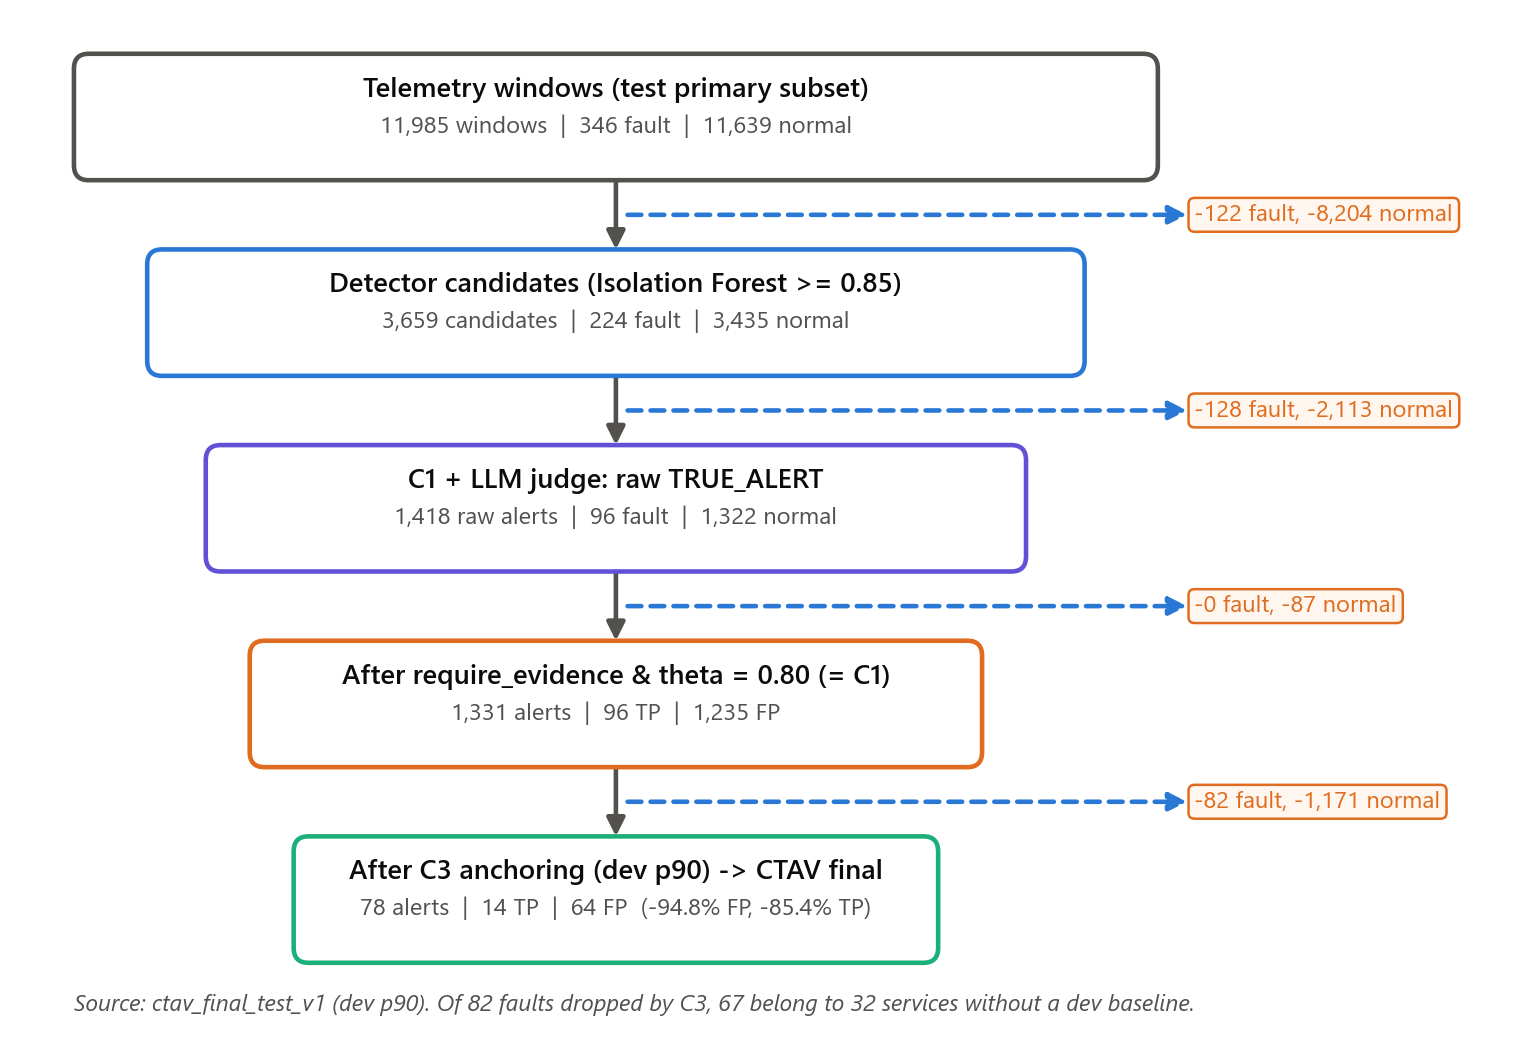
\includegraphics[width=\linewidth]{figures/ch5/h5.11-ctav-funnel-test.png}
  \caption[Phễu quyết định của CTAV trên tập test]{Phễu quyết định của \CTAV{} trên $11.985$ cửa sổ có telemetry của \splitname{test}, cho thấy tầng C3 cắt $94{,}8\%$ FP nhưng đồng thời hạ $82$ TP (trong đó $67$ TP thuộc các service thiếu ngưỡng \splitname{dev}). \emph{(Nguồn: tác giả vẽ, có hỗ trợ AI.)}}
  \label{fig:ch5-funnel}
\end{figure}

Bảng~\ref{tab:ch5-ablation-both} đối chiếu đầy đủ các biến thể ablation trên \splitname{test} cạnh tham chiếu \splitname{val}. Hai thành phần bị loại (C2, C4) tiếp tục không mang lại lợi ích trên \splitname{test}: mọi phán quyết bị C2 chặn đều đã bị C3 chặn từ trước (McNemar $p = 1{,}000$), còn C4 đẩy tổng số lượt gọi lên $16.985$ (do $10.412$ ca không có ngữ cảnh ở tầng 1 đều leo thang sang tầng 2) mà chỉ phát sinh thêm $4$ FP.

\begin{table}[htbp]
  \centering
  \caption[Bảng ablation thành phần quanh CTAV trên test cạnh val]{Hiệu năng các biến thể ablation quanh \CTAV{} trên \splitname{test} ($11.985$ cửa sổ có telemetry, $346$ lỗi) đối chiếu với \splitname{val}.}
  \label{tab:ch5-ablation-both}
  \scriptsize
  \renewcommand{\arraystretch}{1.15}
  \setlength{\tabcolsep}{2.5pt}
  \begin{tabularx}{\linewidth}{@{}Y r r r c r r r@{}}
    \toprule
    \textbf{Biến thể (\splitname{test})} & \textbf{TP / FP} & \textbf{Prec.} & \textbf{Recall} & \textbf{F1 [CI95]} & \textbf{FPR} & \textbf{USD} & \textbf{\splitname{val} F1} \\
    \midrule
    \textbf{\CTAV{}} (\splitname{dev} $p_{90}$) & 14 / 64 & 0,179 & 0,040 & 0,066 [0,036; 0,100] & 0,0055 & 8,16 & 0,201 \\
    Bỏ C3 (\code{no\_c3} = C1) & 96 / 1.235 & 0,072 & 0,277 & 0,114 [0,093; 0,135] & 0,1061 & 8,16 & 0,126 \\
    + C2 ($\theta_{\text{topo}} = 0{,}85$) & 14 / 64 & 0,179 & 0,040 & 0,066 [0,036; 0,100] & 0,0055 & 8,16 & 0,202 \\
    + C4 (\code{fp\_conf = 0,95}) & 14 / 68 & 0,171 & 0,040 & 0,065 [0,036; 0,099] & 0,0058 & 13,56 & 0,188 \\
    \textbf{C3-trượt} (60 phút $p_{90}$) & \textbf{47 / 391} & \textbf{0,107} & \textbf{0,136} & \textbf{0,120 [0,090; 0,151]} & \textbf{0,0336} & 8,16 & 0,137 \\
    \bottomrule
  \end{tabularx}
\end{table}

\subsection{Độ phủ ngưỡng nền \splitname{dev} và sự sụt giảm recall (Phát hiện 11)}
\label{sec:ch5-finding11}

Vì sao C3 (\splitname{dev} $p_{90}$) chỉ làm rơi $26/55$ TP trên \splitname{val} nhưng làm rơi tới $82/96$ TP trên \splitname{test}? Bảng~\ref{tab:ch5-finding11} và Hình~\ref{fig:ch5-finding11} tách toàn bộ cửa sổ có telemetry của hai split thành hai nhóm: service có ít nhất một ngưỡng thao tác hợp lệ trong \code{span\_baseline.parquet} (dựng từ $14$ service có cửa sổ bình thường sạch trong \splitname{dev}) và service không có ngưỡng nào. Do phần lớn service trên Nezha không ghi log \code{ERROR}/\code{WARN} trực tiếp lên pod có cửa sổ metric, mọi cảnh báo trên nhóm service thiếu ngưỡng nền \splitname{dev} đều bị C3 hạ về $0$.

\begin{figure}[htbp]
  \centering
  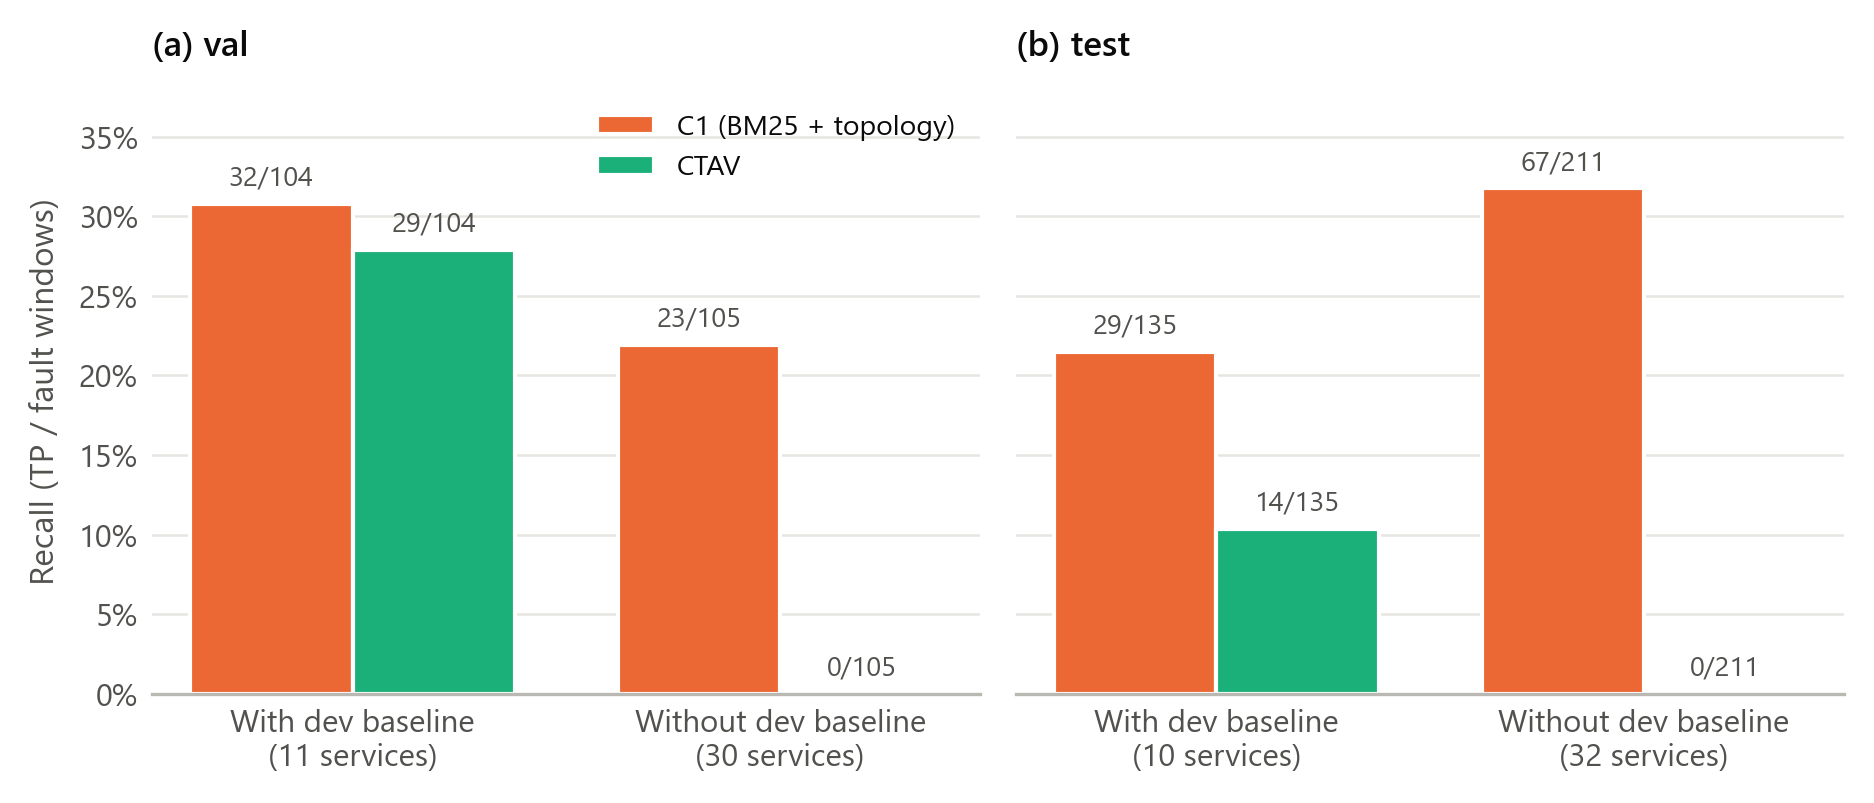
\includegraphics[width=0.92\linewidth]{figures/ch5/h5.12-recall-by-service-group.png}
  \caption[Recall của C1 và CTAV theo nhóm service có và thiếu ngưỡng dev]{Recall của C1 và \CTAV{} tách theo nhóm service có và không có ngưỡng nền \splitname{dev} trên (a)~\splitname{val} và (b)~\splitname{test}; ở nhóm thiếu ngưỡng, \CTAV{} mất trắng $100\%$ TP.}
  \label{fig:ch5-finding11}
\end{figure}

\begin{table}[htbp]
  \centering
  \caption[Phân tách C1 và CTAV theo độ phủ ngưỡng nền dev của service]{So sánh C1 và \CTAV{} (\splitname{dev} $p_{90}$) theo nhóm service có và không có ngưỡng nền \splitname{dev} trên \splitname{val} và \splitname{test}.}
  \label{tab:ch5-finding11}
  \scriptsize
  \renewcommand{\arraystretch}{1.15}
  \begin{tabularx}{\linewidth}{@{}Y r r r r@{}}
    \toprule
    \textbf{Chỉ tiêu (cửa sổ có telemetry)} & \textbf{\splitname{val}: có \splitname{dev}} & \textbf{\splitname{val}: thiếu} & \textbf{\splitname{test}: có \splitname{dev}} & \textbf{\splitname{test}: thiếu} \\
    \midrule
    Số service có cửa sổ telemetry / có lỗi & 11 / 8 & 30 / 10 & 10 / 9 & 32 / 11 \\
    Cửa sổ có telemetry & 1.438 & 6.198 & 1.428 & 10.557 \\
    Cửa sổ lỗi / lỗi là candidate & 104 / 50 & 105 / 59 & 135 / 93 & 211 / 131 \\
    C1: TP / FP & 32 / 290 & 23 / 316 & 29 / 99 & 67 / 1.136 \\
    \CTAV{} (\splitname{dev} $p_{90}$): TP / FP & 29 / 51 & \textbf{0 / 0} & 14 / 64 & \textbf{0 / 0} \\
    Recall C1 & 0,308 & 0,219 & 0,215 & 0,318 \\
    Recall \CTAV{} (\splitname{dev} $p_{90}$) & 0,279 & \textbf{0,000} & 0,104 & \textbf{0,000} \\
    \bottomrule
  \end{tabularx}
\end{table}

Trên \splitname{test}, có tới $88{,}1\%$ cửa sổ telemetry ($10.557/11.985$) và $61{,}0\%$ cửa sổ lỗi ($211/346$) rơi vào $32$ service thiếu ngưỡng \splitname{dev} — gồm hàng loạt service mang nhiều TP nhất của C1 như \code{checkoutservice} ($17$ TP), \code{currencyservice} ($10$), \code{adservice} ($9$), \code{ts-food-service} ($9$), \code{productcatalogservice} ($8$), \code{ts-preserve-service} ($7$) và \code{ts-basic-service} ($5$). Việc hạ trọn $67/67$ TP trên nhóm này làm \CTAV{} mất ngay $0{,}194$ recall toàn tập. Khi thay duy nhất nguồn ngưỡng bằng cửa sổ trượt 60 phút không cần nhãn (\code{C3-trượt}, nâng độ phủ span C1 từ $16{,}1\%$ lên $91{,}2\%$), hệ thống giữ được $47$ TP (nhiều hơn BM25 $13$ TP, tức $+38\%$), cắt $68{,}3\%$ FP của C1 ($1.235 \to 391$, đưa FPR về $0{,}0336$ sát mức $0{,}0317$ của BM25) và đạt F1 cao nhất toàn bảng ($0{,}120$, vượt \CTAV{} đóng băng có ý nghĩa thống kê với $\Delta\text{F1} = +0{,}054$ $[+0{,}017;\, +0{,}091]$, $p < 0{,}001$). Kết quả này chứng minh \emph{nguyên lý neo bằng chứng C3 đúng}, còn sự thất bại của H2 bắt nguồn từ tính mong manh của ngưỡng tĩnh \splitname{dev} trước độ lệch thành phần service.

\subsection{Đường F1 theo ngân sách gọi LLM}
\label{sec:ch5-budget}

Hình~\ref{fig:ch5-budget} và Bảng~\ref{tab:ch5-budget} theo dõi F1 dọc theo các mốc ngân sách $\{120, 250, 500, 1.000, 2.000, 4.000, \text{đủ}\}$ khi duyệt candidate theo thứ tự thời gian. Trên \splitname{test}, \CTAV{} dẫn trước BM25 và LLM-không-RAG ở mốc $120$, nhưng đi ngang quanh $0{,}032$--$0{,}036$ từ mốc $500$ đến $4.000$ rồi mới tăng lên $0{,}066$ ở mức đủ ($13.699$ candidate). Có hai lý do kỹ thuật trực tiếp: (1) giữa mốc $1.001$ và $4.000$, các candidate phát sinh đều rơi vào khoảng chạy nền không có telemetry nên mọi chỉ số không đổi; và (2) toàn bộ $4.000$ candidate đầu tiên nằm trọn trong ngày đầu tiên của OnlineBoutique, nơi phần lớn sự cố sau mốc $120$ thuộc các service thiếu ngưỡng \splitname{dev}, khiến C1 tăng lên $39$ TP ($\text{F1} = 0{,}142$) trong khi \CTAV{} đóng băng dừng ở $7$ TP.

\begin{figure}[htbp]
  \centering
  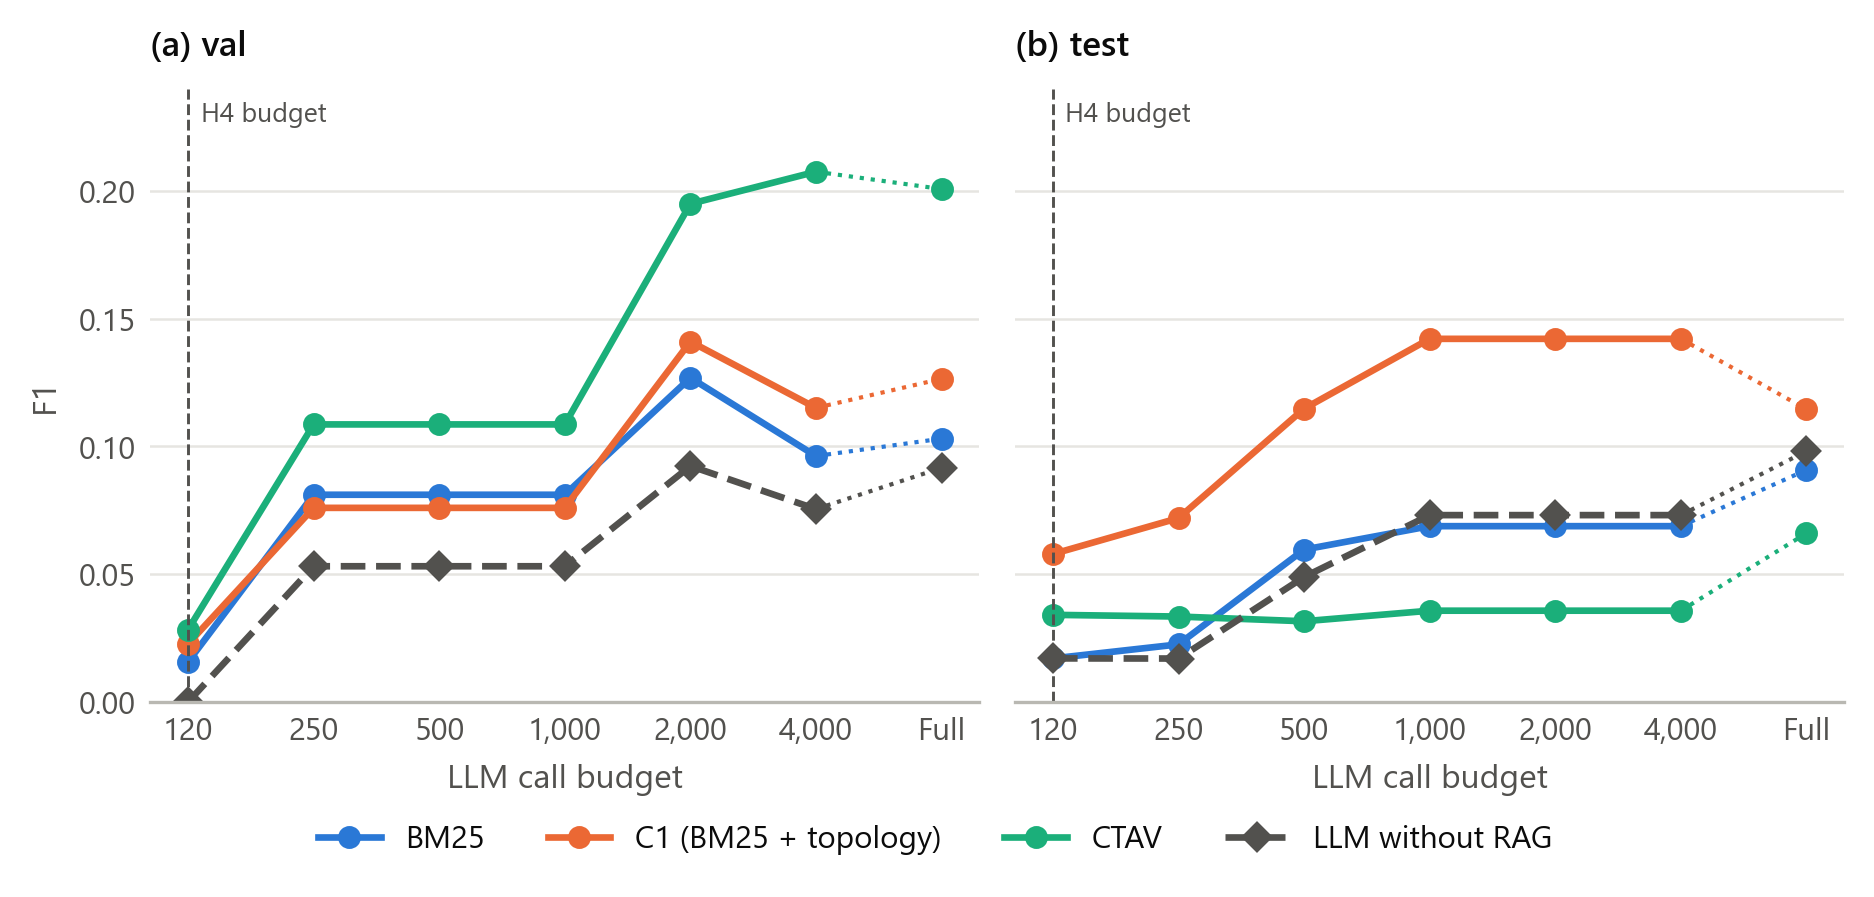
\includegraphics[width=\linewidth]{figures/ch5/h5.13-f1-vs-budget.png}
  \caption[Đường F1 theo ngân sách lần gọi LLM trên val và test]{Đường cong F1 theo ngân sách lượt gọi LLM (thang log, duyệt theo thứ tự thời gian) trên cửa sổ có telemetry của (a)~\splitname{val} và (b)~\splitname{test}; vạch đứt đánh dấu mốc 120 của H4.}
  \label{fig:ch5-budget}
\end{figure}

\begin{table}[htbp]
  \centering
  \caption[Giá trị F1 theo ngân sách lần gọi LLM trên test]{F1 của bốn phương pháp theo các mốc ngân sách lượt gọi LLM trên \splitname{test} ($11.985$ cửa sổ có telemetry, $346$ lỗi; mức đủ $= 13.699$ candidate).}
  \label{tab:ch5-budget}
  \scriptsize
  \renewcommand{\arraystretch}{1.15}
  \begin{tabularx}{\linewidth}{@{}Y r r r r r r r@{}}
    \toprule
    \textbf{Phương pháp} & \textbf{120} & \textbf{250} & \textbf{500} & \textbf{1.000} & \textbf{2.000} & \textbf{4.000} & \textbf{Đủ (13.699)} \\
    \midrule
    \textbf{\CTAV{}} & 0,034 & 0,033 & 0,032 & 0,036 & 0,036 & 0,036 & 0,066 \\
    BM25 & 0,017 & 0,023 & 0,060 & 0,069 & 0,069 & 0,069 & 0,091 \\
    C1 & 0,058 & 0,072 & 0,115 & 0,142 & 0,142 & 0,142 & 0,114 \\
    LLM-không-RAG & 0,017 & 0,017 & 0,049 & 0,073 & 0,073 & 0,073 & 0,098 \\
    \bottomrule
  \end{tabularx}
\end{table}

\subsection{Đánh giá C5 (Rescue) một điểm trên \splitname{test}}
\label{sec:ch5-test-c5}

Giữ nguyên điểm tham số đã chốt trên \splitname{val} ($\eta = (0;\, 0{,}4;\, 0{,}6)$, $\tau = 0{,}8$), cổng Rescue vớt lên $61$ cửa sổ trên \splitname{test} ($3$ lỗi trong $122$ lỗi bị detector bỏ sót và $58$ bình thường; chi phí $0{,}09$ USD). Khi qua C1 và judge, cả $3$ cửa sổ lỗi đều bị judge trả \code{FALSE\_POSITIVE} trước khi tới C3, còn $58$ cửa sổ bình thường phát sinh $1$ FP cuối cùng (Bảng~\ref{tab:ch5-test-c5}; $\Delta\text{F1} = 0{,}000$, McNemar $p = 1{,}000$), xác nhận lại Phát hiện 12 trên dữ liệu độc lập.

\begin{table}[htbp]
  \centering
  \caption[So sánh CTAV và CTAV + C5 một điểm trên val và test]{Ảnh hưởng của cổng cứu cảnh báo C5 tại điểm cố định $\eta = (0;\, 0{,}4;\, 0{,}6)$, $\tau = 0{,}8$ trên cả hai split \splitname{val} và \splitname{test}.}
  \label{tab:ch5-test-c5}
  \scriptsize
  \renewcommand{\arraystretch}{1.15}
  \begin{tabularx}{\linewidth}{@{}Y l r r r r c r@{}}
    \toprule
    \textbf{Biến thể} & \textbf{Split} & \textbf{Cửa sổ cứu} & \textbf{TP} & \textbf{FP} & \textbf{Recall} & \textbf{F1 [CI95]} & \textbf{FPR} \\
    \midrule
    \CTAV{} (tắt C5) & \splitname{val} & 0 & 29 & 51 & 0,139 & 0,201 [0,138; 0,264] & 0,0069 \\
    \CTAV{} + C5 & \splitname{val} & 52 & 31 & 67 & 0,148 & 0,202 [0,143; 0,261] & 0,0090 \\
    \CTAV{} (tắt C5) & \splitname{test} & 0 & 14 & 64 & 0,040 & 0,066 [0,036; 0,100] & 0,0055 \\
    \CTAV{} + C5 & \splitname{test} & 61 & 14 & 65 & 0,040 & 0,066 [0,036; 0,101] & 0,0056 \\
    \bottomrule
  \end{tabularx}
\end{table}

\subsection{Độ ổn định lặp lại của bộ thẩm định và đối chiếu chi phí}
\label{sec:ch5-repeat}

Để đo nhiễu nội tại của \code{gemini-2.5-flash} tại nhiệt độ $0$, hai nhánh BM25 và C1 được gọi lặp độc lập thêm hai lần (\code{repeat} $= 1, 2$) trên cùng mẫu ngẫu nhiên $200$ candidate có telemetry của \splitname{test} ($6$ lỗi, $194$ bình thường, \code{seed = 42}). Bảng~\ref{tab:ch5-repeat} cho thấy độ đồng thuận $3/3$ lần đạt $99{,}0\%$ ở BM25 ($2/200$ cửa sổ bình thường đổi nhãn) và $99{,}5\%$ ở C1 ($1/200$ cửa sổ bình thường đổi nhãn); $0$ cửa sổ lỗi bị lật quyết định ở cả hai nhánh. Biên độ nhiễu $0{,}005$--$0{,}010$ nhỏ hơn một bậc độ lớn so với các hiệu ứng chính ($\Delta\text{Recall} = +0{,}179$, $\Delta\text{FPR} = -0{,}0262$), xác nhận kết luận kiểm định ổn định trước phương sai API. Tổng chi phí G-test đạt $15{,}85$ USD ($23{,}37$ triệu token vào, $3{,}53$ triệu token ra) so với ước tính ban đầu $13{,}00$ USD (vượt $2{,}85$ USD chủ yếu do tỷ lệ prompt có bằng chứng và độ dài chuỗi span của OnlineBoutique trên \splitname{test} lớn hơn \splitname{val}).

\begin{table}[htbp]
  \centering
  \caption[Độ ổn định phán quyết của judge qua ba lần gọi độc lập]{Độ lệch câu trả lời của \code{gemini-2.5-flash} qua \code{repeat} $= 0, 1, 2$ trên mẫu 200 candidate có telemetry của \splitname{test} ($6$ lỗi, $194$ bình thường).}
  \label{tab:ch5-repeat}
  \scriptsize
  \renewcommand{\arraystretch}{1.15}
  \begin{tabularx}{\linewidth}{@{}l r c c Y@{}}
    \toprule
    \textbf{Phương pháp} & \textbf{Mẫu} & \textbf{\code{TRUE\_ALERT} thô (r0 / r1 / r2)} & \textbf{Cảnh báo cuối (r0 / r1 / r2)} & \textbf{Tỷ lệ lật nhãn [CI95]} \\
    \midrule
    BM25 & 200 & 0,120 / 0,110 / 0,120 (24/22/24) & 0,085 / 0,075 / 0,085 (17/15/17) & 0,010 [0,000; 0,025] (2/200) \\
    C1 & 200 & 0,370 / 0,375 / 0,375 (74/75/75) & 0,335 / 0,340 / 0,340 (67/68/68) & 0,005 [0,000; 0,015] (1/200) \\
    \bottomrule
  \end{tabularx}
\end{table}

\subsection{Đánh giá context precision bằng chấm tay}
\label{sec:ch5-context-precision}

Để đánh giá chất lượng bằng chứng truy xuất độc lập với bộ thẩm định LLM, hệ thống đã trích xuất ngẫu nhiên một mẫu mù gồm $50$ cửa sổ có telemetry trên \splitname{test} ($25$ lỗi, $25$ bình thường, \code{seed = 42}) thành $525$ dòng bằng chứng phân biệt tại \code{eval/manual/context\_precision\_test\_v1.csv}, tách hoàn toàn nhãn phương pháp (BM25 hay C1) và nhãn cửa sổ sang tệp khóa riêng. Quy trình chấm theo thang ba mức (\code{relevant}, \code{irrelevant}, \code{unsure}) sẽ bổ sung số liệu hoàn chỉnh vào Bảng~\ref{tab:ch5-ctx-prec} sau khi hoàn tất phiên chấm tay.

\begin{table}[htbp]
  \centering
  \caption[Khung bảng đánh giá context precision chấm tay trên mẫu 50 cửa sổ test]{Khung tổng hợp \emph{context precision} chấm tay trên mẫu mù 50 cửa sổ có telemetry của \splitname{test} (25 lỗi, 25 bình thường; 525 dòng bằng chứng).}
  \label{tab:ch5-ctx-prec}
  \scriptsize
  \renewcommand{\arraystretch}{1.15}
  \begin{tabularx}{\linewidth}{@{}l Y c c c c@{}}
    \toprule
    \textbf{Phương pháp} & \textbf{Nhóm cửa sổ} & \textbf{Số bằng chứng} & \textbf{Liên quan} & \textbf{Không liên quan} & \textbf{Context precision} \\
    \midrule
    BM25 & Lỗi (25) / Bình thường (25) & \multicolumn{4}{c}{\CHO{chấm tay}{525 dòng trong \code{context\_precision\_test\_v1.csv}}} \\
    C1 & Lỗi (25) / Bình thường (25) & \multicolumn{4}{c}{\CHO{chấm tay}{525 dòng trong \code{context\_precision\_test\_v1.csv}}} \\
    \bottomrule
  \end{tabularx}
\end{table}

% -----------------------------------------------------------------------------
\section{Đánh giá tác tử RCA (H5)}
\label{sec:ch5-rca}

Mục này trình bày kết quả lựa chọn tham số tác tử RCA trên \splitname{val} và kiểm định chính thức giả thuyết H5 trên tập \splitname{test}.

\subsection{Chọn tham số trên \splitname{val} và thiết lập kiểm định H5}
\label{sec:ch5-rca-setup}

Trên $80$ cảnh báo của \CTAV{} trên \splitname{val}, hệ thống quét $T_{\text{group}} \in \{180, 300, 600\}\,\text{s}$ theo quy tắc định trước (ưu tiên tối thiểu số sự cố đa lỗi nhập nhằng \code{ambiguous} rồi đến ARR). Mức $T_{\text{group}} = 180\,\text{s}$ được chọn vì tạo $1$ sự cố \code{ambiguous} so với $2$ sự cố ở $300\,\text{s}$ và $600\,\text{s}$ (ARR mọi cảnh báo đạt $0{,}675$; Hit@1 mức 1 bằng baseline $= 7/11 = 0{,}636$; JSON valid rate $26/26 = 1{,}000$; riêng ARR trên \code{network\_delay} chỉ đạt $0{,}250$ do thiếu cảnh báo đầu vào). Cấu hình chốt (\code{eval/configs/rca\_final.yaml}, dấu vân tay \code{b0c54fa68ef65535}) được sao nguyên sang \splitname{test} để chạy một lần lên đúng $78$ cảnh báo của \CTAV{} đóng băng. Ngoài kết quả đăng ký chính thức, một dòng \emph{độ nhạy ngoài bản đăng ký} được chạy trên $438$ cảnh báo của \code{c3\_rolling\_baseline} để tách ảnh hưởng của độ phủ cảnh báo đầu vào khỏi bản thân thuật toán định vị; dòng độ nhạy chỉ mang tính phân tích và không dùng thay đổi kết luận H5.

\subsection{Kết quả kiểm định H5 trên \splitname{test}}
\label{sec:ch5-rca-results}

Bảng~\ref{tab:ch5-h5} đối chiếu bốn vế đã đăng ký của H5 trên \splitname{test} ($78$ cảnh báo $\to$ $38$ sự cố, gồm $17$ sự cố có nhãn đơn lỗi, $3$ sự cố \code{ambiguous} và $18$ sự cố không ứng với lỗi nào). Bảng~\ref{tab:ch5-rca-compare} đặt song song ba lượt chạy (\splitname{val}, \splitname{test} đăng ký và \splitname{test} độ nhạy), còn Bảng~\ref{tab:ch5-rca-by-fault} phân rã kết quả theo năm loại lỗi tiêm.

\begin{table}[htbp]
  \centering
  \caption[Kiểm định giả thuyết H5 trên tập test theo bản đăng ký]{Kết quả kiểm định H5 trên tập \splitname{test} theo cấu hình đăng ký ($78$ cảnh báo \CTAV{} $\to$ $38$ sự cố, $17$ sự cố có nhãn).}
  \label{tab:ch5-h5}
  \scriptsize
  \renewcommand{\arraystretch}{1.15}
  \begin{tabularx}{\linewidth}{@{}Y >{\raggedright\arraybackslash}p{4.4cm} c l@{}}
    \toprule
    \textbf{Vế tiêu chí H5} & \textbf{Số đo trên \splitname{test}} & \textbf{CI95} & \textbf{Kết quả} \\
    \midrule
    $\text{Hit@1} \ge 0{,}60$ & $8 / 17 = 0{,}471$ & $[0{,}235;\, 0{,}706]$ & \textbf{Không đạt} \\
    $\text{Hit@3} \ge 0{,}80$ & $8 / 17 = 0{,}471$ & $[0{,}235;\, 0{,}706]$ & \textbf{Không đạt} \\
    Cận dưới CI95 $\Delta\text{Hit@1}(\text{RCA}-\text{baseline}) > 0$ & $0{,}000$ (baseline $8/17$; $0$ cặp lệch) & $[0{,}000;\, 0{,}000]$ & \textbf{Không đạt} \\
    Alert Reduction $\ge 30\%$ trên cascade & Không tính được ($0/50$ lần tiêm là cascade) & -- & \textbf{Không đạt} \\
    \bottomrule
  \end{tabularx}
\end{table}

\textbf{H5 không được chấp nhận trên tập \splitname{test} (0/4 vế đạt).} Để tham chiếu, tỷ lệ giảm cảnh báo chung (ARR mọi cảnh báo) đạt $0{,}513$ $[0{,}362;\, 0{,}626]$ và trên cảnh báo trong khoảng lỗi đạt $0{,}556$ $[0{,}382;\, 0{,}674]$, nhưng hai chỉ số này không phải tiêu chí cascade đã đăng ký.

\begin{table}[htbp]
  \centering
  \caption[So sánh tác tử RCA trên val, test đăng ký và dòng độ nhạy]{Đối chiếu tác tử RCA trên \splitname{val}, \splitname{test} đăng ký (\CTAV{} \splitname{dev} $p_{90}$) và dòng độ nhạy ngoài đăng ký (\code{c3\_rolling\_baseline}).}
  \label{tab:ch5-rca-compare}
  \scriptsize
  \renewcommand{\arraystretch}{1.15}
  \setlength{\tabcolsep}{3pt}
  \begin{tabularx}{\linewidth}{@{}Y >{\raggedright\arraybackslash}p{2.9cm} >{\raggedright\arraybackslash}p{3.0cm} >{\raggedright\arraybackslash}p{3.1cm}@{}}
    \toprule
    \textbf{Chỉ số} & \textbf{\splitname{val}} & \textbf{\splitname{test} (đăng ký)} & \textbf{\splitname{test} (độ nhạy, ngoài ĐK)} \\
    \midrule
    Cảnh báo vào / số service & 80 / 8 & 78 / 5 & 438 / 22 \\
    Lần tiêm: tổng / có nhãn / 0 cảnh báo & 30 / 10 / 18 & 50 / 17 / \textbf{29} & 50 / 34 / 1 \\
    Sự cố: tổng / có nhãn / mơ hồ / không lỗi & 26 / 11 / 1 / 14 & 38 / 17 / 3 / 18 & 114 / 48 / 14 / 52 \\
    Sự cố nhiều service & 1 & \textbf{0} & 39 \\
    Hit@1 mức 1 & 0,636 [0,364; 0,909] & \textbf{0,471 [0,235; 0,706]} & 0,208 [0,104; 0,333] \\
    Hit@3 mức 1 & 0,636 [0,364; 0,909] & \textbf{0,471 [0,235; 0,706]} & 0,313 [0,188; 0,458] \\
    Hit@1 baseline / $\Delta\text{Hit@1}$ & 0,636 / 0,000 & 0,471 / \textbf{0,000} & 0,229 / $-0{,}021$ \\
    Hit@1 trên mọi lần tiêm lỗi & 0,200 [0,067; 0,333] & 0,160 [0,060; 0,280] & 0,200 [0,100; 0,320] \\
    ARR mọi cảnh báo & 0,675 [0,600; 0,730] & 0,513 [0,362; 0,626] & 0,740 [0,654; 0,796] \\
    ARR cascade (số lần tiêm cascade) & 0,667 (1) & -- (0) & 0,704 [0,591; 0,777] (41) \\
    JSON valid rate & 26 / 26 (1,000) & \textbf{38 / 38 (1,000)} & 114 / 114 (1,000) \\
    \bottomrule
  \end{tabularx}
\end{table}

\begin{table}[htbp]
  \centering
  \caption[Phân rã kết quả định vị RCA theo loại lỗi trên tập test]{Kết quả định vị service gốc theo năm loại lỗi tiêm trên tập \splitname{test} đăng ký ($50$ lần tiêm lỗi).}
  \label{tab:ch5-rca-by-fault}
  \scriptsize
  \renewcommand{\arraystretch}{1.15}
  \begin{tabularx}{\linewidth}{@{}Y r r r r r@{}}
    \toprule
    \textbf{Loại lỗi tiêm} & \textbf{Lần tiêm} & \textbf{0 cảnh báo} & \textbf{Chỉ ở mơ hồ} & \textbf{Sự cố có nhãn} & \textbf{Trúng hạng 1} \\
    \midrule
    \code{network\_delay} & 15 & 5 & 2 & 8 & 2 \\
    \code{cpu\_contention} & 11 & 5 & 1 & 5 & 3 \\
    \code{exception} & 10 & 7 & 0 & 3 & 3 \\
    \code{return} & 9 & 8 & 0 & 1 & 0 \\
    \code{cpu\_consumed} & 5 & 4 & 1 & 0 & -- \\
    \midrule
    \textbf{Tổng cộng} & \textbf{50} & \textbf{29} & \textbf{4} & \textbf{17} & \textbf{8} \\
    \bottomrule
  \end{tabularx}
\end{table}

\subsection{Phân tích nguyên nhân và chất lượng báo cáo JSON}
\label{sec:ch5-rca-analysis}

Cả bốn vế không đạt của H5 quy về cùng một nguyên nhân cấu trúc: \emph{cảnh báo đầu vào hiếm khi rơi đúng vào service gốc}. Trên tập đăng ký, $78$ cảnh báo chỉ phân bố trên $5$ service có ngưỡng nền \splitname{dev} (Phát hiện 11), khiến $29/50$ lần tiêm lỗi không có bất kỳ cảnh báo nào để định vị và toàn bộ $38$ sự cố đều là sự cố một service. Khi một sự cố chỉ chứa một service, thuật toán lan truyền ngược 1 bước trùng tuyệt đối với baseline ($\Delta\text{Hit@1} = 0$, $\text{Hit@3} = \text{Hit@1}$) và không có lỗi cascade để đo ARR. Chín sự cố trượt đều cùng một mẫu: cảnh báo phát ra ở service gọi phía trước (\code{frontend} hoặc \code{ts-travel-service}), còn lỗi tiêm nằm ở service phía sau không phát cảnh báo.

Dòng độ nhạy ($438$ cảnh báo trên $22$ service, $39$ sự cố nhiều service) cho thấy nguyên nhân này không tự mất đi khi tăng số lượng cảnh báo: dù ARR trên $41$ lỗi cascade đạt $0{,}704$ $[0{,}591;\, 0{,}777]$, trong $48$ sự cố có nhãn chỉ có đúng $15$ sự cố chứa service gốc thật trong tập service phát cảnh báo — đặt trần tuyệt đối $15/48 = 0{,}313$ cho mọi thuật toán xếp hạng chỉ nhìn trên tập service đã cảnh báo ($\text{Hit@1} = 0{,}208$, thấp hơn baseline $0{,}021$). Về tầng sinh báo cáo, bộ kiểm duyệt năm quy tắc đạt tỷ lệ JSON hợp lệ $100\%$ ở mọi lượt chạy ($26/26$ trên \splitname{val}, $38/38$ trên \splitname{test} đăng ký, $114/114$ ở độ nhạy; lọc sạch các định danh bằng chứng bịa đặt trong $1$ và $4$ báo cáo), song trường phân loại \code{fault\_type} thiên mạnh về \code{cpu\_contention} ($35/38$ báo cáo) — vấn đề chất lượng nội dung này sẽ được phân tích sâu cùng đánh giá mù bởi con người ở Chương~\ref{ch:thao-luan}.

% -----------------------------------------------------------------------------
\section{Tổng hợp mười hai phát hiện thực nghiệm}
\label{sec:ch5-synthesis}

Xuyên suốt quá trình kiểm chứng từ cổng tái lập đến tập \splitname{test} độc lập, đề tài ghi nhận mười hai phát hiện thực nghiệm nối kết trực tiếp lý thuyết với các quyết định thiết kế và giới hạn hệ thống, hệ thống hóa ở Bảng~\ref{tab:ch5-findings}. Bốn nhóm bài học cốt lõi nổi lên rõ rệt: (1) giao thức dữ liệu quyết định mạnh biên độ chỉ số tuyệt đối (Phát hiện 1--4); (2) bộ thẩm định LLM nhạy cảm với các tín hiệu định dạng như cột metric hằng lỗi và với bằng chứng trace sát $t_0$ bất kể nhãn (Phát hiện 5--7); (3) neo bằng chứng C3 là thành phần duy nhất kìm hiệu quả báo động giả, trong khi C2, C4, C5 không đóng góp (Phát hiện 9, 12); và (4) cách ước lượng ngưỡng nền tĩnh từ một split nhỏ (\splitname{dev}) là nút thắt quyết định khiến cấu hình đóng băng đánh mất recall trên \splitname{test}, qua đó kéo theo việc tác tử RCA thiếu cảnh báo ở service gốc (Phát hiện 8, 10, 11).

\begin{table}[htbp]
  \centering
  \caption[Tổng hợp 12 phát hiện thực nghiệm và vai trò trong đề tài]{Tổng hợp 12 phát hiện thực nghiệm xuyên suốt quá trình đánh giá và tác động thiết kế tương ứng.}
  \label{tab:ch5-findings}
  \scriptsize
  \renewcommand{\arraystretch}{1.15}
  \setlength{\tabcolsep}{3.5pt}
  \begin{tabularx}{\linewidth}{@{}r Y >{\raggedright\arraybackslash}p{4.2cm}@{}}
    \toprule
    \textbf{\#} & \textbf{Phát hiện thực nghiệm} & \textbf{Tác động thiết kế / đánh giá} \\
    \midrule
    1 & Trên Nezha, có bằng chứng gần như tương đương với gần sự cố ($100\%$ lỗi so với $\approx 25\%$ bình thường có telemetry) & Chốt tập chấm chính trên cửa sổ có telemetry (Mục~\ref{sec:ch5-data}) \\
    2 & Độ tin cậy của judge khi thiếu ngữ cảnh chủ yếu sao chép lại \code{anomaly\_score} & Không dùng \code{confidence} thô làm tín hiệu hiệu chỉnh duy nhất \\
    3 & Biến thể ``topology'' trên tập mẫu cũ gần giống BM25 không giới hạn thời gian & Giới hạn kho tìm kiếm trong biên $\pm 8$ phút (\code{bm25\_pool = window}) \\
    4 & Công thức C1 chuẩn không tự đưa bằng chứng lân cận vào top-6 khi không có hạn ngạch & Tách khảo sát C1-quota và H0 trên \splitname{val} \\
    5 & Cột \code{PodSuccessRate(\%)} luôn bằng $0$ khiến judge không bác bỏ cảnh báo & Thêm tham số \code{drop\_metrics} loại cột hằng lỗi (Mục~\ref{sec:ch4-judge}) \\
    6 & Thay đổi trọng số Fusion $(\alpha, \beta, \gamma)$ không điều khiển tỷ lệ bằng chứng lân cận & Giữ bộ trọng số chuẩn $(0{,}35;\, 0{,}25;\, 0{,}40)$ và $k_{\text{graph}} = 0$ \\
    7 & H0 tái lập hiện tượng tăng Recall \& FPR nhưng nguyên nhân là trace cục bộ sát $t_0$, không phải nhiễu lân cận & Định hình lại H1 và chuyển trục chính sách sang neo bằng chứng tại $s_0$ \\
    8 & Ngưỡng nền \splitname{dev} $p_{90}$ chỉ phủ $31{,}8\%$--$33{,}2\%$ span trên \splitname{val} ($16{,}1\%$ trên \splitname{test}) & Đưa biến thể \code{C3-trượt} 60 phút vào H3 để đối chứng \\
    9 & Tầng 1 BM25 sinh nhiều FP và tỷ lệ leo thang lớn khiến C4 tốn chi phí hơn C1 chạy thẳng & Loại C4 khỏi cấu hình \CTAV{} chốt (xác nhận lại trên \splitname{test}) \\
    10 & \CTAV{} cắt $91{,}6\%$--$94{,}8\%$ FP nhưng không giữ được recall của C1 & Báo cáo trung thực kết luận H2, không nới tiêu chí đăng ký \\
    11 & Ngưỡng \splitname{dev} gây ``im lặng có cấu trúc'' trên $32/42$ service của \splitname{test} (mất $67/96$ TP của C1) & Giải thích trực tiếp kết quả H2, H5 và khẳng định ưu thế của \code{C3-trượt} \\
    12 & Cổng cứu C5 chỉ thêm $\le 2$ TP trên \splitname{val} và $+0$ TP / $+1$ FP trên \splitname{test} (nút thắt ở judge) & Giữ C5 làm kết quả ablation âm, không bật trong pipeline chính \\
    \bottomrule
  \end{tabularx}
\end{table}

% -----------------------------------------------------------------------------
\section{Kết chương}
\label{sec:ch5-ket-chuong}

Chương này đã hoàn tất kiểm định định lượng toàn bộ hệ thống trên ba lớp bằng chứng độc lập: vượt qua hai cổng kỹ thuật G-port và G-paper ($100\%$ cache hit), tinh chỉnh và đóng băng cấu hình trên \splitname{val}, rồi kiểm định một lần duy nhất trên tập \splitname{test} niêm phong. Theo đúng tiêu chí đã đăng ký trước: \textbf{H0 được chấp nhận} (4/4 vế, xác nhận đánh đổi Recall--FPR của C1); \textbf{H1 được giữ một phần} trên \splitname{val} (chỉ ra độ nhạy chung với trace cục bộ sát $t_0$); \textbf{H2 không được chấp nhận} trên \splitname{test} (đạt sâu vế giảm FPR $5{,}8$ lần so với BM25 nhưng mất recall do $32/42$ service thiếu ngưỡng nền \splitname{dev}, trong khi đối chứng \code{C3-trượt} 60 phút nâng F1 lên $0{,}120$); \textbf{H3 được chấp nhận} (khẳng định C3 là đóng góp lõi và xác nhận loại C2, C4, giữ C5 làm ablation âm); \textbf{H4 được chấp nhận} ở mốc $120$ lượt gọi; và \textbf{H5 không được chấp nhận} (0/4 vế do cảnh báo đầu vào thưa và hiếm rơi vào service gốc, dù JSON valid rate đạt $100\%$ và ARR cascade ở dòng độ nhạy đạt $0{,}704$). Các kết quả và công cụ kiểm chứng này được tích hợp trực tiếp vào nền tảng trình diễn ở Chương~\ref{ch:platform} và phân tích sâu nguyên nhân ca sai ở Chương~\ref{ch:thao-luan}.
